%! TEX root = main.tex
\section{Equazioni struttura stellare}\linkdest{stellarmodel}

\begin{wordonframe}{da fare: kippenhahn wiegert}
\begin{itemize}
\item strutture autogravitanti 1-62' (43). EQuilibrio idrostatico, vento stellare, stabilit\'a e pulsazioni: ho iniziato da succo
\item metodi numerici 77'-84(44-48): sposto nella parte solve
\item esistenza e unicit\'a 85'-99'(48-56)
\item Properties of stellar matter: ideal gas with radiation, ionization, degenerate electron gas, equazione di stato, opacit\'a 102'-144'(57-78)
\item produzione energia reazioni nucleari:  146'-172'(79-92)
\item politrope 174'-190' (93-102)
\end{itemize}
\end{wordonframe}

\subsection{Struttura di equilibrio}\linkdest{stellarstructure}

\begin{frame}{Equazioni struttura di equilibrio (Euleriane)}
\begin{align*}
&\TDy{r}{m}=4\pi r^2\rho\\
&\TDy{r}{P}=-\frac{\rho Gm}{r^2}\overbrace{[-\rho\PtwoDy{t}{r}]}^{\tau_{hyd}=\frac{1}{2}(G\exv{\rho})\expy{-1/2}}\\
&\TDy{r}{T}=\nabla\frac{T}{P}\TDy{r}{P},\ \nrad{}:-\frac{F_r}{c}\kappa_R\rho\,dr=\frac{4}{3}aT^3\,dT\\
&\TDy{r}{L}=4\pi r^2\rho[\epsilon-\epsilon_{\nu} \underbrace{-c_P(\TDy{t}{T}-\nad\frac{T}{P}\TDy{t}{P})}_{\epsilon_g=-T\PDy{t}{s}=-c_P\PDy{t}{T}+\frac{\delta}{\rho}\PDy{t}{P}}]\\
&\TDy{t}{q}=\TDof{t}\underbrace{[du+Pdv]}_{c_P\,dT-\frac{\delta}{\rho}\,dP}=\underbrace{\TDy{t}{u}+P\TDof{t}(\frac{1}{\rho})}_{c_P\TDy{t}{T}-\frac{\delta}{\rho}\TDy{t}{P}}(=\underbrace{\epsilon-\frac{1}{\rho}\nabla\cdot\vec{F})}_{\epsilon-\epsilon_{\nu}+\epsilon_g-\PDy{(4\pi/3r^3\rho)}{l}}=\epsilon+\epsilon_g-\epsilon_{\nu}-\frac{1}{\rho}\frac{1}{r^2}\PDof{r}(r^2F)\\
&\epsilon_g=-T\PDy{t}{s}=-c_P\PDy{t}{T}+\frac{\delta}{\rho}\PDy{t}{P}=-c_PT(\frac{1}{T}\PDy{t}{T}-\frac{\nabla_{Ad}}{P}\PDy{t}{P})\quad(\left(\nabla_{Ad}=\PDly{P}{T}\right)_s=\frac{P\delta}{T\rho c_P})\\
%&\TDy{t}{X_s}\frac{1}{A_s}=\sum_{production}\rho^{n_h+n_k-1}n_p\frac{X_h^{n_h}X_k^{n_k}}{A_h^{n_h}A_k^{n_k}}\frac{\exv{\sigma v}_{hk}}{m_H^{n_h+n_k-1}n_h!n_k!}\tag{$n_hh+n_kk\to n_ps$}\\
%&-\sum_{distruction}\rho^{n_d+n_j-1}n_d\frac{X_s^{n_d}X_j^{n_j}}{A_s^{n_d}A_j^{n_j}}\frac{\exv{\sigma v}_{sj}}{m_H^{n_d+n_j-1}n_d!n_j!}\tag{$n_jj+n_ds\to n_zz$}
&\rho\PDy{t}{X_i}=A_im_H[\sum_j(r_{ji}-r_{ij})]+\frac{1}{r^2}\PDof{r}[r^2\rho D_T\PDy{r}{X_i}]-\frac{1}{r^2}\PDof{r}[r^2\rho v_i]\tag{nucl+turb.mix+atm.diff}\\
&v_i=D_{i,H}[-\PDy{r}{\ln{X_i}}+K_T\PDy{r}{\ln{T}}+\frac{(Z_i+1)m_Hg}{2K_BT}+\frac{A_im_H}{K_BT}(g_{rad,i}-g)]\tag{trace el. i}\\
&v_2-v_1=-D_{12}\{\frac{n^2}{n_1n_2}\nabla\left(\frac{n_1}{n_2}\right)+\frac{m_1-m_2}{\mu}\nabla\ln{P}+\frac{n^2}{n_1n_2}\frac{D_{TH}}{D_{12}}\nabla\ln{T}-\frac{m_1m_2}{\mu K_BT}(F_2-F_1)\}\tag{bin.mixt.}
\end{align*}
\end{frame}

\begin{frame}{Equazioni struttura di equilibrio (Lagrangiane)}
\begin{align*}
&\TDy{m}{r}=\frac{1}{4\pi r^2\rho}\\
&\TDy{m}{P}=-\frac{Gm}{4\pi r^4}\overbrace{[-\frac{1}{4\pi r^2}\PtwoDy{t}{r}]}^{\tau_{hyd}=\frac{1}{2}(G\exv{\rho})\expy{-1/2}}\\
&\TDy{m}{T}=-\nabla\frac{T}{P}\frac{Gm}{4\pi r^4}\\
&\TDy{m}{L}=\epsilon-\epsilon_{\nu} \underbrace{-c_P[\TDy{t}{T}-\nad\frac{T}{P}\TDy{t}{P}]}_{-c_P\PDy{t}{T}+\frac{\delta}{\rho}\PDy{t}{P}}\quad(\TDy{t}{q}=\underbrace{\TDy{t}{u}+P\TDof{t}(\frac{1}{\rho})}_{c_P\TDy{t}{T}-\frac{\delta}{\rho}\TDy{t}{P}}=\underbrace{\epsilon-\frac{1}{\rho}\nabla\cdot\vec{F})}_{\epsilon-\PDy{m}{l}}\\
&\TDy{t}{X_s}\frac{1}{A_s}=\sum_{production}\rho^{n_h+n_k-1}n_p\frac{X_h^{n_h}X_k^{n_k}}{A_h^{n_h}A_k^{n_k}}\frac{\exv{\sigma v}_{hk}}{m_H^{n_h+n_k-1}n_h!n_k!}\tag{$n_hh+n_kk\to n_ps$}\\
&-\sum_{distruction}\rho^{n_d+n_j-1}n_d\frac{X_s^{n_d}X_j^{n_j}}{A_s^{n_d}A_j^{n_j}}\frac{\exv{\sigma v}_{sj}}{m_H^{n_d+n_j-1}n_d!n_j!}\tag{$n_jj+n_ds\to n_zz$}
\end{align*}
\end{frame}

\begin{frame}{Conservazione massa e HE}
\begin{columns}[T]
	\begin{column}{0.5\textwidth}
\begin{align*}
&\frac{D\rho}{Dt}=\PDy{t}{\rho}+(\scap{v}{\nabla})\rho\tag{mat-dev}\\
&\frac{D\rho}{Dt}=\rho\scap{\nabla}{v}\tag{Lagr. mass cont.}\\
&\PDy{t}{\rho}+\nabla\cdot(\rho\vec{v})=0\tag{Euler mass cont.}\\
&\TDy{m}{r}=\frac{1}{4\pi r^2\rho}\\
&\frac{D\vec{v}}{Dt}=-\nabla\Omega-\frac{1}{\rho}\nabla P[+\frac{1}{\rho}\div{\tau}]\\
&\TDy{m}{P}=-\frac{Gm}{4\pi r^4}\overbrace{[-\frac{1}{4\pi r^2}\PtwoDy{t}{r}]}^{\tau_{hyd}=\frac{1}{2}(G\exv{\rho})\expy{-1/2}}\\
&\tau_{hyd}=\sqrt{\frac{R^3}{GM}}
\end{align*}
\end{column}\begin{column}{0.5\textwidth}
\begin{align*}
&\TDy{r}{m}=4\pi r^2\rho\\
&\TDy{r}{P}=-\frac{Gm}{r^2}\rho\overbrace{[-\rho\PtwoDy{t}{r}]}^{\tau_{hyd}=\frac{1}{2}(G\exv{\rho})\expy{-1/2}}\\
&\tau_{ff}=\sqrt{\frac{R}{g}}\\
&\tau_{exp}=R\sqrt{\frac{\rho}{P}}
\end{align*}
\end{column}
\end{columns}
Red giant: $\tau_H\approx\SI{5}{\day}$ (time for the shock to cross a supergiant star making a SNII, Cepheid); Sun: $\tau_H\approx\SI{38}{\minute}$; WD: $\tau_H\approx\SI{2}{\second}$
\end{frame}

\begin{frame}{Trasporto energia verso la superficie e gradiente termico}
    \begin{columns}[T]
        \begin{column}{0.6\textwidth}
    \begin{align*}
        &\TDy{s}{I_{\nu}}=j_{\nu}\rho-\kappa_{\nu}\rho I_{\nu}\xrightarrow{\times\cos{\theta}\times\int\,d\Omega}\underbrace{\int_{\Omega}\PDy{r}{I}\cos^2{\theta}\,d\Omega}_{=c\PDy{r}{P_{rad}}}-\underbrace{\int_{\Omega}\frac{1}{r}\PDy{r}{I}\cos{\theta}\sin{\theta}\,d\Omega}_{\frac{c}{r}(3P_{rad}-u)}\\
        &=\int_{\Omega}\rho j\cos{\theta}\,d\Omega-\int_{\Omega}\rho\kappa I\cos{\theta}\,d\Omega\\
        &\TDof{s}=\PDof{r}\TDy{s}{r}+\PDof{\theta}\TDy{s}{\theta}=\PDof{r}\cos{\theta}-\frac{\sin{\theta}}{r}\PDof{\theta}\xrightarrow{\mu=\cos{\theta}}\mu\PDof{r}+\invers{r}(1-\mu^2)\PDof{\theta}
    \end{align*}
        \end{column}
        \begin{column}{0.4\textwidth}
            \begin{figure}[!ht]
                \centering
                 %trim={<left> <lower> <right> <upper>}
                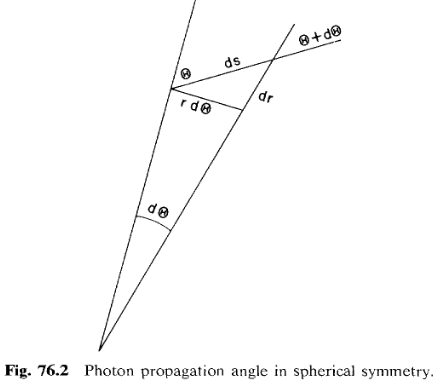
\includegraphics[trim={2.5cm 1cm 3cm 0.5cm},clip, keepaspectratio,width=0.4\textwidth]{radtransfspheric}
                \label{fig:gradalongray}
            \end{figure}
        \end{column}
    \end{columns}
    
    \begin{columns}[T]
        \begin{column}{0.7\textwidth}
\begin{align*}
&dP_{rad}=-dp=-\frac{dF_{Rad}}{c}=-\frac{F_{rad}}{c}\frac{dr}{l}=-\frac{F_{rad}}{c}\kappa_R\rho\,dr=\frac{4}{3}aT^3dT\\
&dP_{rad}(\nu)=-\frac{F_{rad}(\nu)}{c}\kappa_{\nu}\rho\,dr=\frac{4\pi}{3c}\TDy{r}{B_{\nu}(T)}\,dr
\end{align*}
        \end{column}
        \begin{column}{0.3\textwidth}
\begin{align*}
&B_{\nu}(T)=\frac{2h\nu^3}{c^2}\frac{1}{\exp{\frac{h\nu}{kT}}-1}
\end{align*}
        \end{column}
    \end{columns}

\begin{columns}[T]
	\begin{column}{0.6\textwidth}
		\begin{align*}
		&\TDy{m}{T}=-\nabla\frac{T}{p}\frac{Gm}{4\pi r^4}\\
		&\nabla=\nrad=\frac{3\kappa_R}{16\pi acG}\frac{LP}{mT^4}\tag*{$\nrad\leq\nad$}\\
		&\nabla=\nad+\Delta\nabla\tag*{$\nrad>\nad-\frac{\chi_{\mu}}{\chi_T}\nmu$}
		\end{align*}
	\end{column}\begin{column}{0.4\textwidth}
		\begin{align*}
		&\TDy{r}{T}=\nabla\frac{T}{P}\TDy{r}{P}\\
		&\nabla=\TDly{P}{T}
		\end{align*}
	\end{column}
\end{columns}
\begin{columns}[T]
	\begin{column}{0.6\textwidth}
		\begin{align*}
		&\TDy{m}{T}=-\nabla\frac{T}{P}\frac{Gm}{4\pi r^4}\\
		&\nabla=\nrad=\frac{3\kappa_R}{16\pi acG}\frac{LP}{mT^4}\tag*{$\nrad\leq\nad$}\\
		&\nabla=\nad+\Delta\nabla\tag*{$\nrad>\nad-\frac{\chi_{\mu}}{\chi_T}\nmu$}
		\end{align*}
	\end{column}\begin{column}{0.4\textwidth}
		\begin{align*}
		&\TDy{r}{T}=\nabla\frac{T}{P}\TDy{r}{P}\\
		&\nabla=\TDly{P}{T}
		\end{align*}
	\end{column}
\end{columns}
\end{frame}


\begin{frame}{Equazioni struttura stellare: conservazione energia - Luminosit\'a}
\begin{columns}[T]
\begin{column}{0.4\textwidth}
\begin{align*}
&\TDy{m}{L}=\epsilon-\epsilon_{\nu} \underbrace{-c_P[\TDy{t}{T}-\nad\frac{T}{P}\TDy{t}{P}]}_{-c_P\PDy{t}{T}+\frac{\delta}{\rho}\PDy{t}{P}0-T\PDy{t}{s}}\\
&\epsilon_{gr}=-T\PDy{t}{s}=-\TDof{t}u+\frac{P}{\rho^2}\TDy{t}{\rho}\\
&\epsilon_{gr}>0\tag*{contrazione}\\
\epsilon_{\nu}&=\Pelectron\APelectron\to\Pneutrino\APneutrino\tag{Pair annihilation}\\
&=\Pgamma\Pepm\to\Pepm\Pneutrino\APneutrino\tag{Photoproduction}\\
&=\Pgammastar\to\Pneutrino\APneutrino\tag{Plasmon decay}\\
&=\Pepm Z\to\Pepm Z\Pneutrino\APneutrino\tag{Bremsstahlung}\\
    \end{align*}

\end{column}\begin{column}{0.6\textwidth}
\begin{align*}
&\TDy{r}{L}=4\pi r^2[\rho(\epsilon-\epsilon_{\nu})-\rho\TDof{t}u+\frac{P}{\rho}\TDy{t}{\rho}]\\
&
\end{align*}
\begin{figure}[!ht]
            \centering
            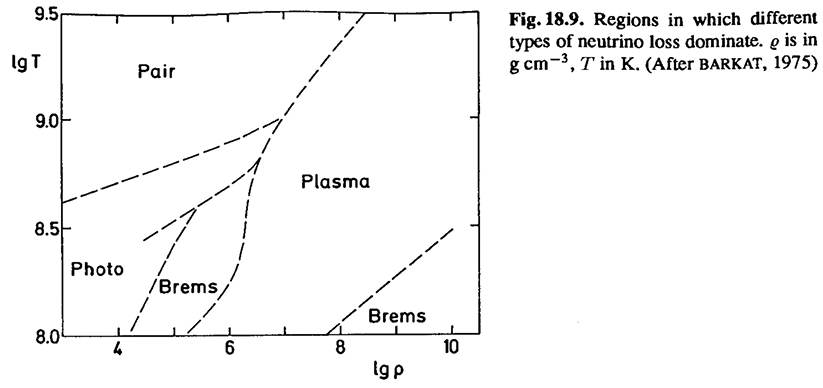
\includegraphics[trim={0cm 0cm 0cm 0cm},clip, keepaspectratio,width=0.9\textwidth]{nucreation}
            %\caption{}
            \label{fig:nucreation}
        \end{figure}
\end{column}
\end{columns}
\end{frame}

\begin{frame}{Chemical evolution: nuclear burning, diffusion and convective mixing}\linkdest{diffusion}\
    \begin{columns}[T]
        \begin{column}{0.3\textwidth}
            \begin{block}{Nucl. Chem Evol.}
            $X_i$ frazione in massa dell'elemento s: $\sum_sX_s=1$: $i+j\to k$,$r_{ij}=\frac{N_iN_j}{1+\delta_{ij}}\exv{v\sigma}_{ij}$ is number reaction per unit volume and time, $R_{ij}=r_{ij}/\rho$ is number of reactions per unit time and mass
            \begin{align*} 
                &\TDy{t}{X_i}=-A_im_HR_{ij}\\
                &=-\rho \frac{X_iX_j}{m_HA_j}\frac{\exv{v\sigma}_{ij}}{1+\delta_{ij}}
            \end{align*}
        \end{block}
        \end{column}
        \begin{column}{0.7\textwidth}
            \begin{block}{Cycle}
                    \begin{align*}
                        &a+b\to c\\
                        &c+b\to a\\
                        &X_a=X_a^0\exp{-Pt}+X_a^{\infty}(1-\exp{-Pt})
                    \end{align*}
                    If $X_b\gg X_a,X_c$ and $\tau_{eq}=\frac{1}{P}\ll\tau_{dyn}$: $\rho, X_b$ approx const
                \end{block}
                \begin{block}{Fully mixed convective shell ($\tau_{X_i}=\frac{1}{X_i}\dot{X_i}\gg\tau_{conv}$)}
                    \begin{align*}
                        &\TDy{t}{\exv{X_i}}=\frac{1}{\Delta m}[\int_{m_1}^{m_2}\TDy{t}{X_i}\,dm+\TDy{t}{m_2}(X_{i2}-\exv{X_i})-\TDy{t}{m_1}(X_{i1}-\exv{X_i})]\\
                        &\Delta m=m_2-m_1
                    \end{align*}
                    $X_{i1},X_{i2}$ abb. on radiative side at inner/outer boundary.
                \end{block}
        \end{column}
    \end{columns}
    \begin{block}{Atomic diffusion: Chapman-Enskog Theory}
        Total distribution function an be written as a convergent serie $f_i(\vec{r},\vec{v},t)=\underbrace{f_i^{(0)}(\vec{r},\vec{v},t)}_{\text{Maxwell}}+f_i^{(1)}(\vec{r},\vec{v},t)+\ldots$ then substitute into Boltzmann equation and linearize: Transport coeff. are obtained from first order approximation of distribution.
    \end{block}
\end{frame}

\begin{frame}{Cyclic reactions}
    \begin{columns}[T]
        \begin{column}{0.3\textwidth}
            \begin{align*}
                &a+b\to c\\
                &c+b\to a\\
                &A=\frac{\rho X_bA_a}{m_HA_cA_b}\\
                &B=\frac{\rho X_b}{m_HA_b}\\
                &
            \end{align*}
            c,a secondary, b primary; $\rho, X_b$ approx const ($X_b\gg X_a,X_c$, $\tau_{eq}=\frac{1}{P}\ll\tau_{dyn}$): $A,B$ const; Sum of abb in numbers of a,c is conserved: $\frac{X_a}{A_a}+\frac{X_c}{A_c}=\frac{X_a^0}{A_a}+\frac{X_c^0}{A_c}=K^0$, quindi $X_c=A_cK_0-\frac{A_cX_a}{A_a}$. Equilibrium abundances:
            \begin{align*}
                &X_a^{\infty}=\frac{K^0A_cA\exv{cb}}{P}\\
                &X_c^{\infty}=\frac{K^0A_cB\exv{\sigma v}_{ab}}{P}\\
                &\tau_{eq}\sim \frac{1}{P}
            \end{align*}

        \end{column}
        \begin{column}{0.7\textwidth}
            \begin{align*}
                &\dot{X_a}=\rho[\frac{X_cX_bA_a}{m_HA_cA_b}\exv{\sigma v}_{cb}-\frac{X_aX_b}{m_HA_b}\exv{\sigma v}_{ab}]\\
                &\dot{X_c}=\rho[\frac{X_aX_bA_c}{m_HA_aA_b}\exv{\sigma v}_{ab}-\frac{X_cX_b}{m_HA_b}\exv{\sigma v}_{cb}]\\
                &\Rightarrow\dot{X}_a=X_cA\exv{\sigma v}_{cb}-X_aB\exv{\sigma v}_{ab}\\
                &\dot{X}_a=K^0A_cA\exv{\sigma v}_{cb}-X_a(\frac{A_cA}{A_a}\exv{\sigma v}_{cb}+B\exv{\sigma v}_{ab})\\
                &=-PX_a+K^0A_cA\exv{\sigma v}_{cb}\\
                &X_a=X_a^0\exp{-Pt}+X_a^{\infty}(1-\exp{-Pt})
            \end{align*}
        \end{column}
    \end{columns}
\end{frame}

\subsection{Considerazioni energetiche}\linkdest{virialstability}

\begin{frame}{Teorema del viriale}
\begin{columns}[T]
	\begin{column}{0.45\textwidth}
		\begin{align*}
&\Omega=-\int_0^M\frac{Gm(r)}{r}\,dm\\
&\frac{1}{2}\TtwoDy{t}{I}=2E_i+\Omega\tag{T. viriale}\\
&0=2\int_M\frac{3}{2}\frac{P}{\rho}\,dm(r)+\Omega\tag{stationary}\\
&E_i=\frac{1}{\gamma-1}\frac{P}{\rho}\\
&\frac{P}{\rho}=\frac{R}{\mu}T=(c_P-c_v)T=(\gamma-1)c_vT\xrightarrow{\text{Id. mon.: } \gamma=\frac{5}{3}}\frac{2}{3}u\\
&\zeta u=3 \frac{P}{\rho}\tag{General EOS: ideal $\zeta=3(\gamma-1)$}
		\end{align*}
	\end{column}\begin{column}{0.55\textwidth}
		\begin{align*}
&W=E_i+\Omega \tag{total E}\\
&\TDy{t}{W}+L=0\tag{E conservation}\\
&L=-\frac{1}{2}\dot{\Omega}=\dot{E}_i\\
&\frac{1}{2}\TtwoDy{t}{I}=3(\gamma-1)W-(3\gamma-4)\Omega\\
&E_T=E_i+\Omega=\frac{3\gamma-4}{3(\gamma-1)}\Omega\\
&\gamma>4/3\tag{stability}
		\end{align*}
	\end{column}
\end{columns}
Nel caso in cui la contrazione gravitazionale sia l'unica fonte di energia per una massa gassosa in equilibrio idrostatico, il suo tempo di evoluzione caratteristico \'e il tempo di \kh{} $\tkh{}=\frac{\Omega}{L}\approx\frac{GM^2}{2RL}$
\end{frame}

\begin{frame}{Core contraction-shell expansion (astrocollins)}

\end{frame}

\frameinlbftrue
\begin{frame}{Stability: What happens for $\gamma<\frac{4}{3}$}

	\begin{itemize}
		\item Dynamical stability: $P=\int_m^M\frac{mG}{4\pi r^4}\,dm$ - assuming homologous adiabatic compression we have from HE $\frac{P'}{P}=(\frac{R'}{R})^{-4}$ and $\frac{P'}{P}=(\frac{\rho'}{\rho})^{\gamma_{ad}}=(\frac{R'}{R})^{-3\gamma_{ad}}$ - so for $\gamma_{ad}>\frac{4}{3}$: pressure increases more than weight, for $\gamma_{ad}<\frac{4}{3}$ star would collapse
		\end{itemize}
	
\end{frame}
\frameinlbffalse
    
%\begin{frame}{Relazione massa, densit\'a, temperatura/ massa, peso molecolare, opacit\'a}
%\end{frame}
\section{Trasporto}\linkdest{transport}

\subsection{Trasporto radiativo: cos'\'e $\nabla=\nabla_{rad}$?}\linkdest{trarad}

\begin{frame}{Caratteristiche del gas di fotoni}
    \begin{itemize}
        \item Intensity (Macroscopic): energy transported $dE=I(\vec{x},t;\vec{n},\nu)dS\cos{\alpha}d\Omega d\nu dt$, $\alpha$: angolo tra $\vec{n}$ e $d\vec{S}$
        \item Photon number density (Microscopic) $\psi$: $\psi(\vec{x},t;\vec{n},\nu)d\Omega d\nu$ number photons traveling around solid angle centered at $\vec{n}$, number of photons crossing $dS$: $\psi(\vec{n}\cdot d\vec{S}d\Omega d\nu cdt$, $dE=ch\nu\psi dS\cos{\alpha}d\Omega d\nu dt$: $I=\psi ch\nu$
        \item photon distro function $f_R$: $f_R(\vec{x},t;\vec{n},p)d^3p$: number of photons per unit volume with moment $[\vec{p},\vec{p}+dp]$, $d^3p=p^2dpd\Omega=(\frac{h}{c})^3\nu^2d\Omega d\nu$: $I=\frac{h^4\nu^3}{c^2}f_R$
        \item Mean intensity (zeroth moment of radiation field over angles): $J_{\nu}=J(\vec{x},t;\nu)=\invers{(4\pi)}\oint I\,d\Omega$ (\si{\erg\per\squared\cm\per\second\per\hertz\per\ster})
    \end{itemize}
\end{frame}

\begin{frame}{Radiative transport}
    \begin{columns}[T]
        \begin{column}{0.5\textwidth}
            \begin{align*}
                &I(\theta)\,d\Omega=cu(\theta)\,d\Omega\\
                &u=\int^{4\pi}u(\theta)\,d\Omega=\frac{1}{c}\int I(\theta)\,d\Omega\tag{Energy density}\\
                &J(\vec{r},\nu,t)=\invers{(4\pi)}\int I(\vec{r},\hat{n},\nu,t)\,d\Omega\tag{Mean Intensity}\\
                &P_r=\frac{1}{3}\int_0^{\infty}\frac{h\nu}{c}cn(\nu)\,d\nu=\frac{1}{3}u\tag{rad Press}\\
                &P_r=\frac{1}{c}\int I(\theta)\cos^2{\theta}\,d\Omega\tag{Rad Press}\\
                &=\int^{4\pi}\frac{I(\theta)\cos{\theta}}{c}\cos{\theta}\,d\Omega\\
                &=\frac{2\pi}{c}\int_0^{2\pi}I(\theta)\cos{\theta}\sin{\theta}\,d\theta\\
                &H=\int I(\theta)\cos{\theta}\,d\Omega\\
                &=2\pi\int_0^{\pi}I(\theta)\cos{\theta}\sin{\theta}\,d\theta\tag{Net En. Flux polar dir}
            \end{align*}
        \end{column}
        \begin{column}{0.4\textwidth}
            Pressione di radiazione: radiazione contenuta in parallelepipedo di superficie unitaria lunghezza c in direzione $\theta$ (l'asse polare forma con la radiazione un angolo $\theta$) quindi la sezione d'urto geometrica in direzione polare contiene fattore $\cos{\theta}$, la proiezione del momento rispetto alla direzione polare ha un altro $\cos{\theta}$.
        \end{column}
    \end{columns}
\end{frame}

\begin{frame}{Momentum transfer Rad-Mat}
    \begin{columns}[T]
        \begin{column}{0.6\textwidth}
    \begin{align*}
        &dp=\frac{dF_{Rad}}{c}=\frac{F_{Rad}}{c}\frac{dr}{l}\\
        &\TDy{r}{P_{Rad}}=-\frac{\kappa\rho}{c}F_{Rad}\\
        &-\frac{F_{rad}(\nu)}{c}\kappa_{\nu}\rho\,dr=\frac{4\pi}{3c}\TDy{r}{B_{\nu}(T)}\,dr\tag{L-grad T}
    \end{align*}
        \end{column}
        \begin{column}{0.4\textwidth}
            Flux of photons through volume matter at r, flux of energy $F_{rad}$. $dp$ momentum transfered from photons to volume element, $l$ photon mean free path: $\invers{l}=\kappa\rho$, $dp$ opposite of change of $dP_{Rad}$ of pressure exerted by photons over dr
        \end{column}
    \end{columns}
\end{frame}

\begin{frame}{Diffusion Approx: Stellar Interior Near TE}
    \begin{columns}[T]
        \begin{column}{0.5\textwidth}
    \begin{align*}
                &U=aT^4\\
                &''\vec{j}=-D\nabla n''\tag{diffusion}\\
                &D=\frac{1}{3}vl_p\\
                &\vec{F}_{\nu}=-D_{\nu}\nabla U_{\nu}\\
                &D_{\nu}=\frac{1}{3}cl_{\nu}=\frac{c}{3\kappa_{\nu}}\rho
            \end{align*}
        \end{column}
        \begin{column}{0.5\textwidth}
            \begin{align*}
                &I(\theta)=I_0+I_1\cos{\theta}+\ldots\\
                &u=\frac{4\pi}{c}I_0\\
                &H=\frac{4\pi}{3}I_1\\
                &P_r=\frac{4\pi}{3c}I_0
            \end{align*}
        \end{column}
    \end{columns}
    \end{frame}

    \begin{frame}{Trasporto radiativo}
\begin{columns}[T]
	\begin{column}{0.5\textwidth}
Diffusion approx: $F_{\nu}=-D_{\nu}\nabla U_{\nu}$.
Radiative transport - $dp$ momentum trasfer from photons to matter
\begin{align*}
&dp=\frac{dF_r}{c}=\frac{F_r}{c}\frac{dr}{\rho\kappa_r}\\
&dP_r=-\frac{F_r}{c}\frac{dr}{l}\\
&\TDy{r}{P_r}=\frac{4}{3}aT^3\TDy{r}{T}\\
&\TDy{r}{P_{r,\nu}}=-\frac{\kappa_{\nu}\rho}{c}F_{\nu}
\end{align*}
Conduzione elettronica
\begin{align*}
&F_e\approx-N_evl\TDy{r}{E}=-kN_evl\TDy{r}{T}
\end{align*}
\end{column}
\begin{column}{0.5\textwidth}
In LTE:
\begin{align*}
&P_{r,\nu}=\frac{4\pi}{3c}B_{\nu}(T)\\
&\frac{1}{\kappa_R}=\frac{\intzi{}\frac{1}{\kappa_{\nu}}\TDy{T}{B_{\nu}(T)}\,d\nu}{\intzi{}\TDy{T}{B_{\nu}(T)}\,d\nu}\\
&\plankfnu{}
\end {align*}
\end{column}
\end{columns}
\end{frame}

\begin{frame}{Rad transfer - clayton}
\begin{columns}[T]
    \begin{column}{0.4\textwidth}
        \begin{figure}[!ht]
            \centering
            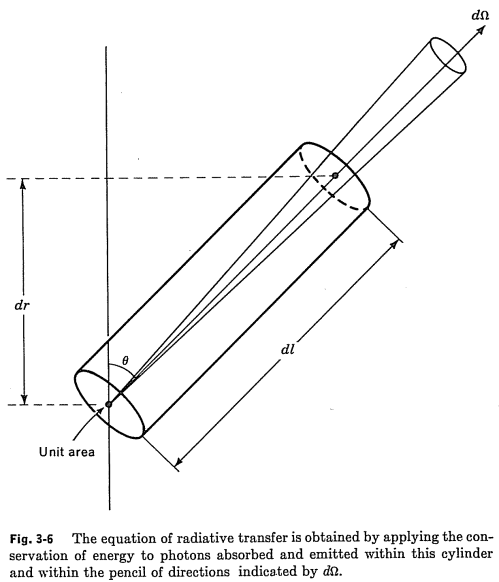
\includegraphics[trim={0cm 0cm 0cm 0cm},clip, keepaspectratio,width=0.9\textwidth]{radtrans-dldr}
            %\caption{}
            \label{fig:clayradransdldr}
        \end{figure}
    \end{column}
    \begin{column}{0.6\textwidth}
        \begin{align*}
            &\frac{1}{\rho dl} \PDy{r}{I}_{\nu}\,dr=\frac{1}{\rho}\PDy{r}{I}_{\nu}\cos{\theta}\\
            &=-(\kappa^*_{\nu,a}+\kappa_{\nu,s})I_{\nu}(r,\theta)+\kappa*_{\nu,a}B_{\nu}(T)\\
            &+\kappa_{\nu,s}\frac{1}{4\pi}\int_{\Omega'}p(\theta\phi;\theta'\phi')I_{\nu}(r,\theta',\phi')\,d\Omega'\\
            &\frac{c}{\rho}\PDy{r}{P}_{\nu}=-(\kappa*_{\nu,s}+\kappa*_{\nu,a})H_{\nu}+0\\
            &+\kappa_{\nu,s}\frac{1}{4\pi}\int_{\Omega}\int_{\Omega'}\cos{\theta}p(\theta,\phi;\theta',\phi')I_{\nu}(r,\theta',\phi')\,d\Omega\,d\Omega'\\
            &\kappa*_{\nu,a}=\kappa_{\nu,a}(1-\exp{\frac{h\nu}{KT}})\tag{reduced absorption}\\
            &H=\int_0^{\infty}H_{\nu}\,d\nu=-\frac{c}{3\rho}\int_0^{\infty}\frac{1}{\kappa_{\nu,a}\kappa_{\nu,s}}\TDy{r}{u_{\nu}}\,d\nu\\
            &=\frac{4ac}{3\kappa\rho}T^3\TDy{r}{T}
        \end{align*}
    \end{column}
\end{columns}

\end{frame}

\subsection{Conduzione}\linkdest{tracond}

\begin{frame}{Diffusione per conduzione}
stima opacit\'a per conduzione gas degenere NR
\end{frame}

\begin{frame}{Conduzione elettronica}
\begin{columns}[T]
\begin{column}{0.5\textwidth}
	\begin{align*}
	&F_e=-N_evl\TDy{r}{E}=-N_ekvl\TDy{r}{T}\\
	&E_T\approx\frac{3}{2}kT,\ v_T\approx\sqrt{\frac{2E_T}{m}}
	\end{align*}
\end{column}
\begin{column}{0.5\textwidth}
	\Pelectron degenerate are forced in higher momentum state - $P_F=2\pi\hbar(\frac{3}{4\pi g})\expy{1/3}n\expy{1/3}$
\end{column}
\end{columns}
\end{frame}

\subsection{Opacit\'a}\linkdest{kapparad}

\begin{frame}{Opacit\'a radiativa (analitico)}
Scattering elettronico, processi ff, fotoionizzazione; opacit\'a atmosfera: ione H-
\end{frame}

\begin{frame}{Andamento opacit\'a: electron scattering e Kramer's opacity (FF)}
\begin{itemize}
\item Electron scattering $\rho\kappa_{\nu}=n_e\frac{8\pi}{3}(\frac{e^2}{m_ec^2})^2=0.2(1+X)\si{\square\cm\per\gram}$ - $\sigma_T=\SI{0.66e-24}{\square\cm}$ - for $T$ maggiore di few milion K is dominant source - Compton scattering $h\nu|_M\gtrsim0.1 m_ec^2$, $h\nu|_M\approx4.96kT$: Compton scattering reduces opacity about $20\%$ for $T>\SI{e8}{\kelvin}$
    \begin{align*}
        &\sigma_T=\frac{8\pi}{3}r_e^2\approx\SI{6.7e-25}{\square\cm},\ \kappa_{\nu}=\sigma_T \frac{n_e}{\rho},\ \mu_e=\frac{2}{1+X},\ \mu_em_u=\frac{\rho}{n_e}:\ \kappa_{\nu}=\frac{\sigma_T}{\mu_em_u}
    \end{align*}
\item Kramers opacity: $T<\SI{e7}{\kelvin}$ -when FF, BF dominates: $\kappa_R\propto\rho T\expy{-7/2}$
\end{itemize}
\begin{block}{Free-free: radiation boost free-\Pelectron from lower to higher state}
Fully ionized-$Z_i$ mixture: 
\begin{align*}
&\rho\kappa_{\nu}(ff)=\sum_in_{Z_i}ne\sqrt{\frac{2m_e}{3\pi kT}}[\frac{4\pi Z_i^2e^6}{3m_e^2ch\nu^3}]g_{ff}(\nu)(1-\exp{-h\nu/kT})\\
&=\num{3.8e22}\overbrace{(X+1)}^{\propto n_e}\overbrace{[X+Y+B]}^{\propto\frac{X}{m_u}+\frac{4Y}{4m_u}+\sum_i\frac{X_iZ_i^2}{A_i}}\ [\si{cgs}]
\end{align*}
$\tau_{\Pelectron-int}\propto\frac{1}{v}\propto T\expy{-1/2}$: \Pelectron experience sharp acceleration $\approx\delta$ resulting in constant emission frequency, two body ion-\Pelectron encounter $\propto n_in_e$, \Pelectron have thermal distro $\propto\exp{-\epsilon/kT}$: $\rho j_{\nu}=n_en_iT\expy{-1/2}\exp{-\frac{h\nu}{kT}}$ - dalla legge di Kirchhoff, $j_{\nu}=4\pi\kappa_{\nu}^{abs}B_{\nu}(T)$, we have $\kappa_{\nu}^{abs}\propto\rho T\expy{-1/2}\nu\expy{-3}[1-\expy{-h\nu/kT}]$
\end{block}
\end{frame}

\begin{frame}{Kramer's opacity (BF, BB) and $H^-$ ions opacity}
\begin{block}{BF}
Hydrogenic atom with charge Z and one \Pelectron in bound state n:
\begin{align*}
&\sigma_{\nu}(Z)=n\expy{-5}\frac{8\pi}{3\sqrt{3}}\frac{Z^4m_ee\expy{10}}{c\hbar^3(h\nu)^3}:\ h\nu>\chi=\frac{Ze^2}{2a_Z}\\
&\rho\kappa_{\nu}(bf)=\sum_in_{Z_i}\sigma_{\nu}(Z_i)(1-\exp{-h\nu/kT})\\
&\kappa_R(bf)=\num{3e25}\underbrace{(1-X-Y)}_{n_{\exv{Z}}}\underbrace{(1+X+\frac{3}{4}Y)}_{n_e}\rho T\expy{-7/2}
\end{align*}
\end{block}
\begin{block}{BB: usually neglected in stellar interior}
\end{block}
\begin{block}{$H^-$ opacity $T<\SIrange{e4}{e5}{\kelvin}$}
BB/BF transition for $H^-$ don't follow Kramer as ion abundance in solar photosphere is sensitive to other considerations: law of mass action for $H^-=H+\Pelectron$ is $\frac{n_{H^-}}{n_Hn_e}=K_1(T)$, and sources of free electrons are metals (Na, K) $M^++\Pelectron=M$ so $\frac{n_{M^+}n_e}{n_M}=K_2(T)$, supposing $n_e=n_{M^+}$:
\begin{align*}
&\rho\kappa_{H^-}^{ff}\propto n_{H^-}n_eT\expy{-7/2}=n_Hn_MT\expy{-7/2}K_1(T)K_2(T)
\end{align*}
\end{block}
\end{frame}

\subsection{Convezione}\linkdest{traconv}

\begin{wordonframe}{Forza di archimede}
Una regione stellare \'e convettivamente stabile se una perturbazione di densit\'a infinitesima non cresce ad ampiezza finita.
\begin{equation*}\label{eq:buoyanc yEOM}
\rho\PtwoDy{t}{(\Delta r)}=-g\Delta\rho=-g[\Dcvar{\TDy{r}{\rho}}{e}-\Dcvar{\TDy{r}{\rho}}{amb}]\Delta r
\end{equation*}
La forza di Archimede ha verso opposta alla perturbazione se
\begin{equation*} 
[\Dcvar{\TDy{r}{\rho}}{e}-\Dcvar{\TDy{r}{\rho}}{amb}]>0
\end{equation*}
Riscrivo prima legge della termodinamica come $dq=c_P\,dT-\frac{\delta}{\rho}\,dP$
\begin{equation*} 
N^2=g(\frac{1}{\Gamma_1P}\TDy{r}{P}-\frac{1}{\rho}\TDy{r}{\rho})=g(\frac{1}{\densityscale{}}-\frac{g}{c_s^2})\label{eq:bvfs}
\end{equation*}
$N^2$ rappresenta la massima frequenza sotto cui pu\'o oscillare una particella di fluido sottoposta a onde di gravit\'a mantenendo l'equilibrio di pressione con l'ambiente.
\begin{equation*}
\PtwoDy{t}{(\Delta r)}=-N^2\Delta r
\end{equation*} 
che descrive un comportamento oscillatorio per $N^2>0$
\end{wordonframe}

\begin{frame}{Convective regions and temperature gradient}
\begin{columns}[T]
	\begin{column}{0.6\textwidth}
\begin{block}{Criterio di \sch e Ledoux: regioni convettive}
	\begin{align*}
	&\rho\PtwoDy{t}{(\Delta r)}=-g\Delta\rho=-g[\Dcvar{\TDy{r}{\rho}}{e}-\Dcvar{\TDy{r}{\rho}}{amb}]\Delta r\\
	&\nrad{}>\nad+\frac{\phi}{\delta}\nmu{}=\nad-\frac{\chi_{\mu}}{\chi_T}\TDly{(P)}{(\mu)}\\
	&\nrad{}>\nad\\
	&\frac{d\rho}{\rho}=\alpha\frac{dP}{P}-\delta\frac{dT}{T}+\phi\frac{d\mu}{\mu}\\
	&=-\frac{\chi_T}{\chi_{\rho}}\frac{\Delta T}{T}-\frac{\chi_{\mu}}{\chi_{\rho}}\frac{\Delta\mu(\Lambda)}{\mu}\\
	&\Delta P=0=\chi_{\rho}\frac{\Delta\rho}{\rho}+\chi_T\frac{\Delta T}{T}+\chi_{\mu}\frac{\Delta\mu}{\mu}
	\end{align*}
\end{block}
	\end{column}
	\begin{column}{0.4\textwidth}
\begin{figure}[!ht]
	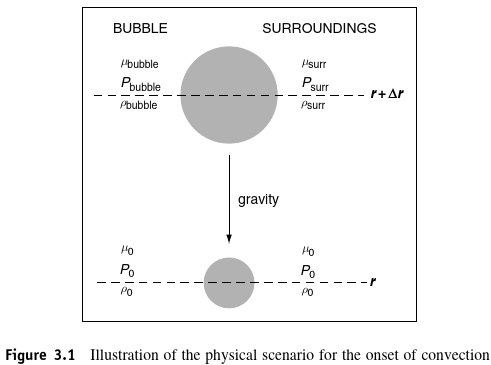
\includegraphics[trim={0cm 0cm 1cm 0cm},clip, keepaspectratio,width=0.99\textwidth]{convectivestability}\label{fig:convectivestability}
\end{figure}
\end{column}\end{columns}
\end{frame}

\begin{frame}{Mixing length: gradiente ambientale e velocit\'a elementi convettivi}
Le stelle con massa $M\leq1.1\msun{}$ hanno una regione radiativa interna mentre la parte esterna \'e convettiva. Convezione esterni $\nabla>\nad$, $v\approx1-10\si{\kilo\meter\per\second}\approx c_s$- $\nabla\to\nad{}$ in interni stellari convettivi: $\TDy{r}{T}=(1-\frac{1}{\Gamma_2})\frac{T}{P}\TDy{r}{P}$, $v\approx\SI{100}{\meter\per\second}\ll c_s$
	\begin{align*}
&F=\frac{L}{4\pi r^2}=F_{rad}+F_{con}=-\frac{4acT^3}{3\kappa\rho}\TDy{r}{T}|_{amb}+\frac{1}{2}\rho vc_p[\TDy{r}{T}|_{Ad}-\TDy{r}{T}|_{amb}]\Lambda\\
&v^2=-\frac{1}{8}g\frac{\Delta\rho}{\rho}\Lambda=\frac{1}{8}g\frac{\Lambda}{H_P}Q(\nabla-\nad),\ Q=1-\TDly{T}{\mu},\ \Lambda=\alpha H_P\\
&F_{con}^{up}=\frac{1}{2}\rho vc_PT\frac{\lambda}{H_P}(\nabla-\nad{})
\end{align*} 
\begin{columns}[T]
\begin{column}{0.3\textwidth}
\begin{align*}
&f_r&=-g\Delta\rho(r)=0\tag{r}\\
&&\propto\Delta r
\end{align*} 
\end{column}
\begin{column}{0.7\textwidth}
Work done per unit volume moving bubble of $\Delta r$
\begin{align*}
&W(\Delta r)=-g\int_0^{\Delta r}\Delta\rho(\Delta r')d(\Delta r')=-\frac{1}{2}g\Delta\rho(\Delta r)\Delta r\\
&\exv{W(\Delta r)}_{\Delta r}=\frac{1}{4}W(\Lambda)=\frac{1}{2}\rho v^2
\end{align*} 
\end{column}\end{columns}
%Calcolo altezza scala di pressione, flusso convettivo e gradiente ambientale in funzione della velocit\'a media degli elementi
\end{frame}

\begin{wordonframe}{EOS e $\nad{}$}
Considero un'equazione di stato generica $\rho(P,T,\mu)$ e definita tramite:
\begin{align*}
&\frac{d\rho}{\rho}=\alpha\frac{dP}{P}-\delta\frac{dT}{T}+\phi\frac{d\mu}{\mu}\\
&P=\frac{\rho\gasconstant{}T}{\mu}\quad\Rightarrow\quad\alpha=\delta=\phi=1
\end{align*}
Definisco le lunghezze caratteristiche per variazione di densit\'a e pressione:
\begin{equation*}
\densityscale{}=-\frac{dr}{d\ln{\rho}},\ H_P=-\frac{dr}{d\ln{P}}
\end{equation*}
e i gradienti termici per il blob, l'ambiente e il gradiente di composizione chimica ambientale
\begin{equation*}
\nabla=\Dcvar{\TDly{P}{T}}{amb},\ \nabla_e=\Dcvar{\TDly{P}{T}}{e},\ \nmu{}=\Dcvar{\TDly{P}{\mu}}{amb}
\end{equation*}
\end{wordonframe}

\begin{wordonframe}{EOS e EOM}
Riscrivo l'equazione del moto utilizzando l'equazione di stato per scrivere la differenza di densit\'a in termini dei gradienti termici e di composizione chimica; inoltre supponendo il moto dell'elemento in equilibrio di pressione con l'ambiente e assumendo $\nmu{}_{blob}\approx0$ risulta:
\begin{equation*}
\PtwoDy{t}{(\Delta r)}=-g\frac{\delta}{H_P}[\nabla_e-\nabla-\frac{\phi}{\delta}\nmu{}]\Delta r
\end{equation*}
\end{wordonframe}

\begin{wordonframe}{Criterio di \sch/Ledoux}
Infine per ricavare il criterio di stabilit\'a per convezione suppongo  il moto del blob adiabatico:
\begin{equation*}
dq=c_P\,dT-\frac{\delta}{\rho}\,dP
\end{equation*}
da cui risulta:
\begin{equation*}
\nabla_e=\nabla_{ad}=\frac{P\delta}{T\rho c_P}
\end{equation*}
cio\'e una regione solare \'e stabile per convezione se
\begin{equation*}
\nrad{}<\nad+\frac{\phi}{\delta}\nmu{}\label{eq:ledoux}
\end{equation*}
dove ho usato $\nabla_{amb}=\nrad{}$, cio\'e il gradiente che si ha nel caso l'energia sia trasportata dai fotoni.
\end{wordonframe}

\subsection{Teoria della mixing-length.}

\begin{wordonframe}{Convezione in esterni stellari}
    \begin{columns}[T]
        \begin{column}{0.5\textwidth}
            \begin{align*}
                &F=F_{con}+F_{rad}=\frac{\lsun{}}{4\pi r^2}\\
                &F_{con}=\exv{\rho vc_P\Delta T}\label{eq:convectiveflux}\tag{Avg on r-sphere}\\
                &\frac{\Delta T}{T}\approx\frac{1}{T}\PDy{r}{(\Delta T)}\underbrace{\frac{l_m}{2}}_{\Delta r\approx\frac{l_m}{2}}=(\nabla-\nabla_e)\frac{l_m}{2}\frac{1}{H_P}\\
                &-g\frac{\Delta\rho}{\rho}\tag{Force/unit mass}\\
                &v^2=g\delta(\nabla-\nabla_e)\frac{l_m^2}{8H_P}\\
                &f=\frac{4acT^3}{3\kappa\rho}|\PDy{n}{T}|\tag{Rad. exchange}\\
                &\PDy{t}{T_e}=-\frac{\lambda}{\rho Vc_P}\\
                &\Dcvar{\TDy{r}{T}}{e}=\Dcvar{\TDy{r}{T}}{ad}-\frac{\lambda}{\rho Vc_Pv}\label{eq:Tchangelength}\tag{$\Delta T$ per unit length by blob}\\
                &|\PDy{n}{T}|\approx\exv{\Delta T}\\
                &\frac{\nabla_e-\nad{}}{\nabla-\nabla_e}=\frac{6acT^3}{\kappa\rho^2c_Pl_mv}
            \end{align*}
        \end{column}
        \begin{column}{0.45\textwidth}
            Eccesso di calore trasportato dai blob $c_P\Delta T$ rispetto all'ambiente, il cui cammino libero medio \'e la mixing-length $l_m=\alpha H_P$, che da luogo al flusso di energia. Assumo la forza di galleggiamento media sia la met\'a di quella alla superficie r ($\exv{\Delta \rho}\approx\frac{\Delta\rho}{2}$) e lo spostamento medio $\frac{l_m}{2}$: assumo che met\'a del lavoro vada in energia cinetica del blob. Il modulo del flusso radiativo \'e proporzionale al gradiente termico in direzione normale alla superficie del blob quindi l'energia scambiata dall'intera superficie S del blob \'e $\lambda=Sf$ che determina, per la prima legge della termodinamica, dato V volume del blob, una variazione di temperatura per unit\'a di tempo. Le 5 equazioni determinano completamente le variabili $F_{rad}, F_{con}, v, \nabla_e, \nabla$ in funzione di $P,T,l(r),m(r),c_P,\nad{},\nrad{},g$.
%Determino il valor medio della differenza di temperatura prendendo come valore caratteristico dello spostamento del blob $\Delta r\approx\frac{l_m}{2}$ (moti in entrambi i versi)
        \end{column}
    \end{columns}
    %Una maggiore efficienza del trasporto convettivo di energia si riflette in una minore differenza tra il gradiente di temperature adiabatico ed effettivo. Il gradiente termico ambientale $\nabla$ e del blob $\nabla_e$ sono determinati inserendo le espressioni per il flusso radiativo e il flusso convettivo in.
cubic equation for $(\nabla-\nabla_e)$
%\begin{figure}[!h]
%   \includegraphics[ width=0.99\textwidth,keepaspectratio]{proportionflux}
%   \subcaption{Profilo radiale (profondit\'a in \si{\kilo\meter}) del flusso convettivo $F_c$ rispetto al flusso totale $F$, della super-adiabaticit\'a $\nabla-\nad{}$ e regioni di ionizzazione idrogeno e $\cel{He}{4}{}{}$. Da \cite{christensen1997effects}.}\label{fluxproportion}
%\includegraphics[keepaspectratio,width=0.9\textwidth]{specificheatnablaa}
%\subcaption{Profilo radiale di $c_P$ e $\nabla_a$: si ha cambiamento di comportamento nelle regioni di ionizzazione parziale di idrogeno ed elio. Da \cite{stix91sun}.}\label{specificheatnablaa}
%\end{figure}
\end{wordonframe}

\begin{wordonframe}{Solution for ML variables}
    \begin{columns}[T]
        \begin{column}{0.5\textwidth}
            \begin{align*}
                &U=\frac{3acT^3}{c_P\rho^2\kappa l_m^2}\sqrt{\frac{8H_P}{g\delta}}\propto\alpha\expy{-2}H_P\expy{-\frac{3}{2}}\\
                &W=\nrad{}-\nad{}\\
                &\Rightarrow\nabla_e-\nad{}=\nabla-\nad{}-(\nabla-\nabla_e)=2U\sqrt{\nabla-\nabla_e}\\
                &(\nabla-\nabla_e)\expy{\frac{3}{2}}=\frac{8}{9}U(\nrad{}-\nabla)\\
                &(\xi-U)^3+\frac{8U}{9}(\xi^2-U^2-W)=0
            \end{align*}
        \end{column}
        \begin{column}{0.4\textwidth}
            Replacing expression for $v^2$ change temperature per unit length converted in grad form we get third eq. Using explicit formula for $F_{con}$ and $F_{con}=\frac{4acG}{3}\frac{T^4m}{\kappa Pr^2}(\nrad{}-\nabla)$ we get fourth eq. We have reduced yhe five equation to two for $\nabla, \nabla_e$, and defining  $\xi$ as positive root of $\xi^2=\nabla-\nad{}+U^2$ and looking at third eq we see that it's a quadratic eq for $\sqrt{\nabla-\nabla_e}$ with sol. $\sqrt{\nabla-\nabla_e}=-U+\xi$ and inserting this in the fourth eq we arrive at cubic for $\xi$ resol for any $U$ and $W$ params.
        \end{column}
    \end{columns}
    
\end{wordonframe}
%\section{From micro-physics to thermodynamics: Equazione di stato, opacit\'a}\linkdest{micro2macro}%to be throw into stellarplasmamodel

%\begin{multicols}{2}%https://newbedev.com/how-to-explicitly-split-long-toc-in-beamer
%   \tableofcontents[currentsection]{cherryframes}
%\end{multicols}

%\begin{multicols}{2}%https://newbedev.com/how-to-explicitly-split-long-toc-in-beamer
%   \tableofcontents[currentsection]{cherryframes}
%\end{multicols}

\section{EXpansion and contraction phases}\linkdest{expcontrphases}

\begin{frame}{Work done by gravity: positive and negative}

\end{frame}


\section{Nuclear Burning}\linkdest{nuclearburning}

\begin{frame}{Sezione d'urto fusione nucleare}
$E$ l'energia cinetica nel centro di massa dei nuclei: $\sigma(E)=\pi\lambdabar^2*P_0(E)*S(E)$
prodotto della sezione d'urto geometrica (nel riferimento del CM: $\sigma\approx\sum_{l=0}^{\frac{R}{\lambdabar}}(2l+1)\pi\lambdabar^2=\pi(R+\lambdabar)^2$
per energie tipiche degli interni stellari approx onda S), della probabilit\'a di attraversamento della barriera coulombiana e del fattore astrofisico. La lunghezza d'onda di de Broglie relativa delle particelle descrive l'indeterminazione sulla posizione nell'urto di due particelle con momento relativo p $\lambdabar=\frac{\hbar}{p}=\frac{\hbar}{\sqrt{2mE}}$.

L'energia potenziale dovuta all'interazione di due nuclei $Z_1$ e $Z_2$ a distanza r contiene un contributo delle altre cariche presenti nel plasma $U=\frac{Z_1Z_2e^2}{r}+U_s(r_{12})$
l'energia potenziale non schermata e contributo della nuvola elettronica: $U_s$ aumenta la probabilit\'a di attraversamento della barriera coulombiana. Fattore moltiplicativo: $f=\exp{-\midfrac{U_0}{KT}}$ dove $U_0=U_s(0)$ poich\'e $r\ll r_D$ e considerando solo la correzione al fattore di penetrazione ($E_G\gg U_0$).

Per determinare $U_0$ considero l'energia potenziale di $Z_1$ e $Z_2$ a distanza $r$
\begin{equation*}
U=Z_2e\int_{\infty}^r\PDy{r_1}{\phi_1}\,dr_1=\frac{Z_1Z_2e^2\exp{-\midfrac{r}{r_D}}}{r},\ U_s=U-\frac{Z_1Z_2e^2}{r}\approx\frac{Z_1Z_2e^2}{r_D}
\end{equation*}
\end{frame}

\begin{frame}{Energia prodotta in reazioni di fusione???}
$S(E)$ descrive l'interazione a livello nucleare: debolmente dipendente dall'energia in assenza di risonanze.
La probabilit\'a di attraversamento della barriera coulombiana: $P_0(E)=\exp{-2\pi\eta},\ \eta=\sqrt{\frac{m}{2}}\frac{Z_1Z_2e^2}{\hbar E\expy{\frac{1}{2}}}$
Per i nuclei di carica $Z_1$, $Z_2$ e m massa ridotta: $\sigma(E)=\frac{S(E)}{E}\exp{-2\pi\eta}$
Il rate per coppia di particelle
\begin{equation*}
\exv{\sigma v}=\num{1.3005e-15}[\frac{Z_1Z_2}{AT_6^2}]\expy{\frac{1}{3}}fS_{eff}\exp{-\tau}\si{\cubic\cm\per\second},\ \tau=\frac{3E_G}{kT}\approx\num{42.487}(Z_1^2Z_2^2AT_6\expy{-1})\expy{\frac{1}{3}}
\end{equation*}
$S_{eff}$ \'e il risultato dell'espansione dell'integrando per $\invers{\tau}\ll1$ ed estrapolato a $E_G$ a partire dal valore $S(0)$ determinato dalla fisica nucleare.
La funzione $\epsilon(\rho,T,X_i)$ \'e determinata dalla somma di tutti i contributi
\begin{equation*}
\epsilon_{ij}=Q_{ij}\frac{n_in_j}{\rho(1+\delta_{ij})}\lambda_{ij}=\frac{1}{1+\delta_{ij}}Q_{ij}\frac{\rho N_A^2X_jX_k}{{A_iA_j}}\exv{\sigma v}_{ij}\label{eq:energyrate}
\end{equation*}
dove $Q_{ij}$ \'e l'energia liberata per reazione tra nucleo di specie i e j e $\exv{\sigma v}_{ij}$ \'e il rate di reazione per coppia di particelle, mediata su MB- distro
$f(E)dE\propto\frac{E\expy{\frac{1}{2}}}{(kT)\expy{\frac{3}{2}}}\exp{-\frac{E}{kT}}\,dE$:
$S(E)\exp{-\frac{E}{kT}-\frac{b}{\sqrt{E}}}$
ha forma approssimativamente gaussiana il cui massimo $E_G$, energia pi\'u probabile di reazione, e FWHM sono: $E_G=\SI{5.665}{\kilo\ev} A\expy{\frac{1}{3}}T_7\expy{\frac{2}{3}}$ $\Delta E=4.249\si{\kilo\ev}W\expy{\frac{1}{6}}T_7\expy{\frac{5}{6}}$
posto $W=Z_i^2Z_j^2A=Z_i^2Z_j^2\frac{A_iA_j}{A_i+A_j}$.
%\begin{equation*}
%\exv{\sigma v}\propto b\expy{1/3}T\expy{-2/3}\exp{-\frac{b\expy{2/3}}{t\expy{1/3}}}
%\end{equation*}
\end{frame}

\subsection{Catena PP}\linkdest{epsilonpp}

\begin{frame}{PP1: twice $\Pproton(\Pproton,\Pnue\APelectron)d(p,\gamma)^3He$ and $^3He(^3He,2^1H)^4He$}
\begin{columns}[T]
	\begin{column}{0.55\textwidth}
\begin{itemize}
	\item $\tau_p(d)\ll[\tau_{^3He}(d)]_e\ll[\tau_d(d)]_e$: $\frac{\dot{D}}{H}=\frac{H}{2}\exv{\sigma v}_{pp}-H(\frac{D}{H})\exv{\sigma v}_{dp}$ - \keyword{D evolution} $(\frac{D}{H})=\frac{\exv{\sigma v}_{pp}}{2\exv{\sigma v}_{dp}}$, evolution: $(\frac{D}{H})_t=(\frac{D}{H})_e-[(\frac{D}{H})_e-(\frac{D}{H})_0]\exp{-\frac{t}{\tau_p(d)}}$
	\item \keyword{$^3He$ evolution} - $\frac{\dot{^3He}}{H}=\frac{H}{2}\exv{\sigma v}_{pp}-H(\frac{^3He}{H})^2\exv{\sigma v}_{^3He^3He}$ - 
\scalebox{0.8}{	\[\frac{^3He}{H}|_t=0+\sqrt{\frac{\exv{\sigma v}_{pp}}{\exv{\sigma v}_{^3He^3He}}}\tanh(t\sqrt{\frac{H}{2}\exv{\sigma v}_{PP}H\exv{\sigma v}_{^3He^3He}})\]}
\item Produzione energia - $\epsilon_{PPI}^e(T_0=\SI{15}{\mega\ev})(\frac{T}{T_0})\expy{3.9}$
\begin{align*}
&\epsilon_{PPI}=\frac{(6.936-0.265)\si{\mega\ev}H^2\exv{\sigma v}_{pp}}{2\rho}\\
&+\frac{\SI{12.861}{\mega\ev}H^2\exv{\sigma v}_{^3He^3He}}{2\rho}(\frac{^3He}{H})^2\\
&\epsilon_{PPI}^e(T)=6.551N_A\exv{\sigma v}_{PP}(\frac{X_H}{m_H})^2\rho N_A\frac{\si{\mega\ev}}{\si{\second\gram}}
\end{align*}
\end{itemize}
	\end{column}
	\begin{column}{0.45\textwidth}
	\begin{figure}[!ht]
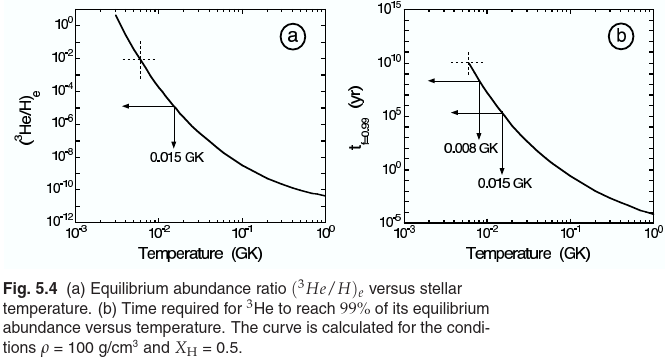
\includegraphics[trim={0cm 0cm 1cm 0cm},clip, keepaspectratio,height=0.28\textheight]{He3eq}
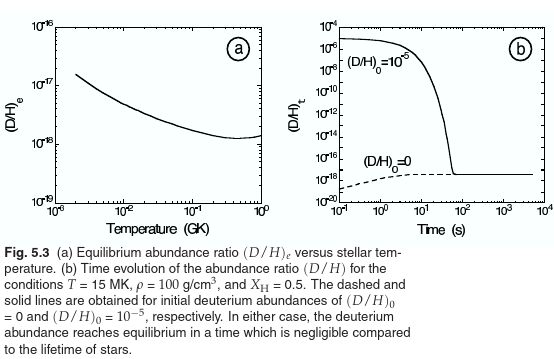
\includegraphics[trim={0cm 0cm 1cm 0cm},clip, keepaspectratio,height=0.28\textheight]{PP1DHet}
\includegraphics[trim={0cm 0cm 1cm 0cm},clip, keepaspectratio,height=0.28\textheight]{pplifetime}
	\end{figure}
	\end{column}
\end{columns}
\end{frame}

\begin{frame}{Network reazioni PP completo}

\begin{columns}[T]
\begin{column}{0.55\textwidth}
Rapid $^8B/^8Be$ decays: $^7Be(p,\gamma)^8B(\APelectron,\nu)^8Be(\alpha)\alpha$ as $^7Be+p\to2\alpha+\gamma$, $\TDof{t}(^7Li+^7Be)\approx0$
\begin{align*}
&Q_{PPI}=27.73-2\exv{E}_{\nu}^{pp}=\SI{26.19}{\mega\ev}\\
&Q_{PPII}=26.73-\exv{E}_{\nu}^{^7Be}-\exv{E}_{\nu}^{pp}=\SI{25.65}{\mega\ev}\\
&Q_{PPIII}=26.73-\exv{E}_{\nu}^{^8B}-\exv{E}_{\nu}^{pp}=\SI{19.75}{\mega\ev}\\
&\epsilon_{PP}=\frac{Q_{4H\to^4He}}{\rho}\dot{^4He}[0.98F_{PPI}+0.96F_{PPII}\\
&+0.74F_{PPIII}],\ f_{PPI}=\frac{r_{^3He^3He}}{r_{^3He^3He}+r_{\alpha^3He}}\\
&F_{PPII}=(1-F_ {PPI})\frac{r_{e^7Be}}{r_{e^7Be}+r_{p^7Be}}
\end{align*}
\end{column}
\begin{column}{0.45\textwidth}
\begin{figure}[!ht]
	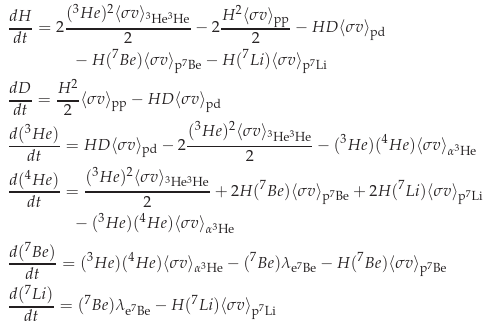
\includegraphics[trim={0cm 0cm 1cm 0cm},clip, keepaspectratio,width=0.72\textwidth]{ppchainsequi}
	\includegraphics[trim={0cm 0cm 1cm 0cm},clip, keepaspectratio,width=0.72\textwidth]{ppfraction}
\end{figure}
\end{column}
\end{columns}
\begin{align*}
&\dot{(^3He)}=\frac{H^2}{2}\exv{\sigma v}_{pp}-2(^3He)^2\frac{\exv{\sigma v}_{^3He^3He}}{2}-(^3He)(^4He)\exv{\sigma v}_{\alpha^3He}\\
&(^3He)_e=\frac{-(^4He)\exv{\sigma v}_{\alpha^3He}+\sqrt{(^4He)^2\exv{\sigma v}_{\alpha^3He}^2+2H^2\exv{\sigma v}_{\alpha^3He}\exv_{\sigma v}_{^3He^3He}}}{2\exv{\sigma v}_{^3He^3He}}
\end{align*}
\end{frame}


\subsection{Ciclo CN-NO:}\linkdest{epsiloncno}

\begin{frame}{Biciclo CNO}
dipendenza da T
flusso neutrini
Modalit\'a combustione H in He: sequenza principale inferiore/superiore
\end{frame}

\begin{frame}{CNOF Network reactions: $4^1H\to^4He+2\APelectron+2\Pnue$}
\begin{columns}[T]
\begin{column}{0.5\textwidth}
\begin{itemize}
\item CNOF elements acts as catalyst: relative initial CNOF abundance are important - produced in previous gen stars at He-burning stages ($^{12}C$, $^{16}O$, less $^{14}N$: solar $^{12}C:^{14}N:^{16}O=10:3:24$)
\item 4 cycle: active cycle influences heavy element abundance - $(p,\gamma)$ compete with $(p,\alpha)$ on $^{15}N$, $^{17}O$, $^{18}$, $^{19}F$: $(p,\alpha)$ faster over entire T-range except $^{17}O$/$^{18}O$ at $T<\SI{20}{\mega\kelvin}$
\item At hydro-burning ($T<\SI{55}{\mega\kelvin}$) much faster than p-induced reactions, at $T>\SI{100}{\mega\kelvin}$ also other reactions are important (HCNO)
\end{itemize}
\end{column}
\begin{column}{0.5\textwidth}
	\begin{figure}[!ht]
	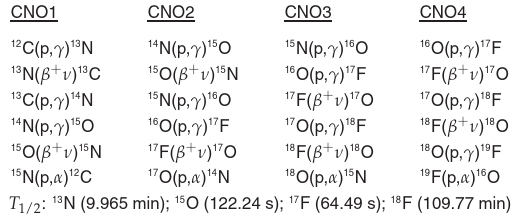
\includegraphics[trim={0cm 0cm 1cm 0cm},clip, keepaspectratio,height=0.28\textheight]{CNO}
	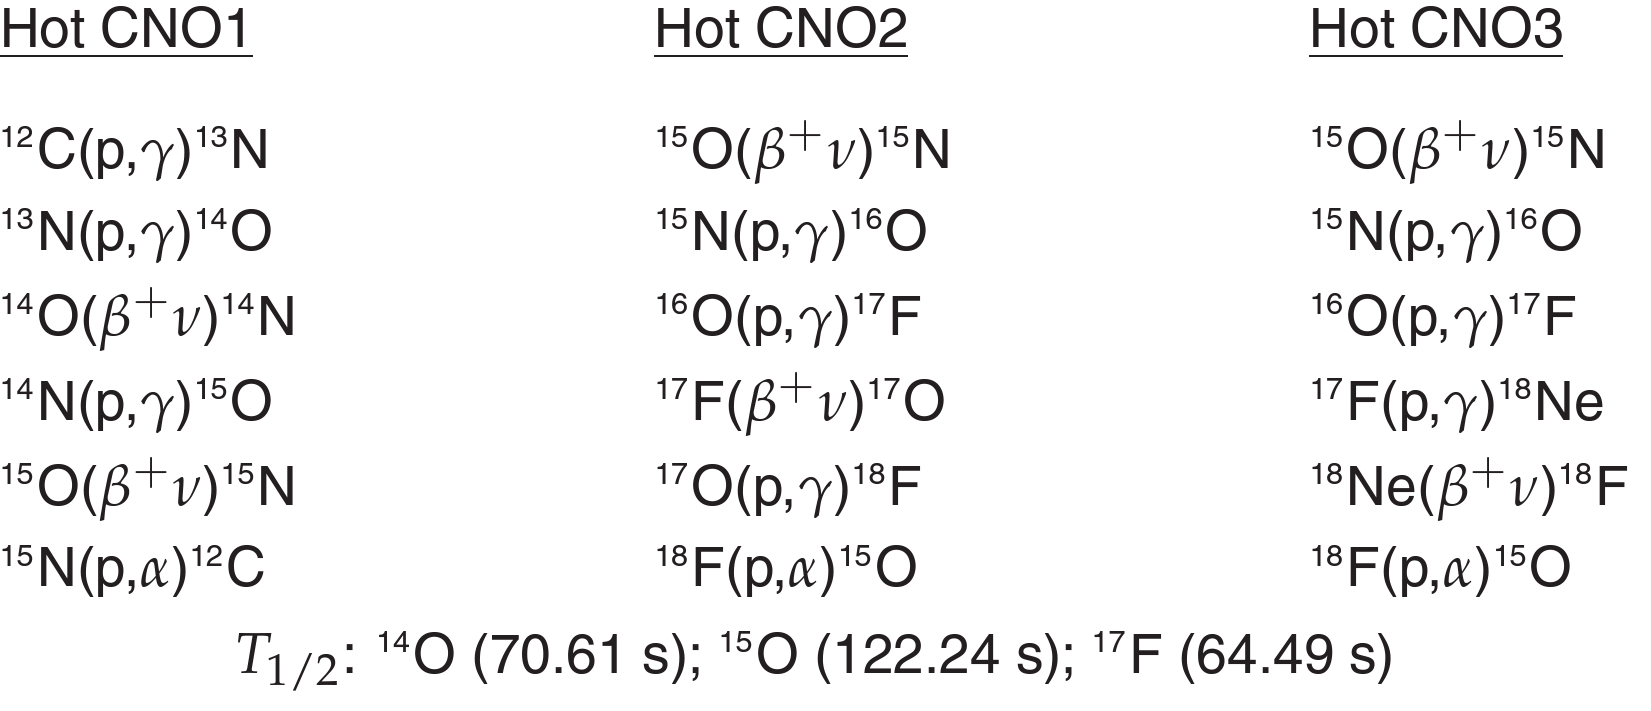
\includegraphics[trim={0cm 0cm 1cm 0cm},clip, keepaspectratio,height=0.28\textheight]{HCNO}
\end{figure}
\end{column}
\end{columns}
\end{frame}

\begin{frame}{CNO1: equilibrium properties}
\begin{columns}[T]
	\begin{column}{0.5\textwidth}
		\begin{itemize}
			\item Elements involving beta-decay reaches equilibrium in few minutes: $\dot{^{13}N}=0$ - $(^{13}N)_t=\frac{\tau_{\beta}(^{13}N)}{\tau_p{^{12}C}}^{12}C[1-\exp{-\frac{t}{\tau_{\beta}(^{13}N)}}]$ - $(\frac{^{13}N}{^{12}C})_e=\frac{\tau_{\beta}(^{13}N)}{\tau_p(^{12}C)}$
			\item At equilibrium ratio of abundance of $^{12}C$, $^{13}C$, $^{14}N$, $^{15}N$ are given by inverse ratio of reaction time (ie $(\frac{^{14}N}{^{12}C})_e=\frac{\exv{\sigma v}_{^{12}C(p,\gamma)}}{\exv{\sigma v}_{^{14}N(p,\gamma)}}=\frac{\tau_p(^{14}N)}{\tau_p(^{12}C)}$), fractional abundance $\frac{(^{12}C)_e}{\sum CNO1}=\frac{\tau_p(^{12}C)}{\tau_p(^{12}C)+\tau_p(^{13}C)+\tau_p(^{14}N)+\tau_p(^{15}N)}$
		\end{itemize}
	\end{column}
	\begin{column}{0.5\textwidth}
		\begin{figure}[!ht]
			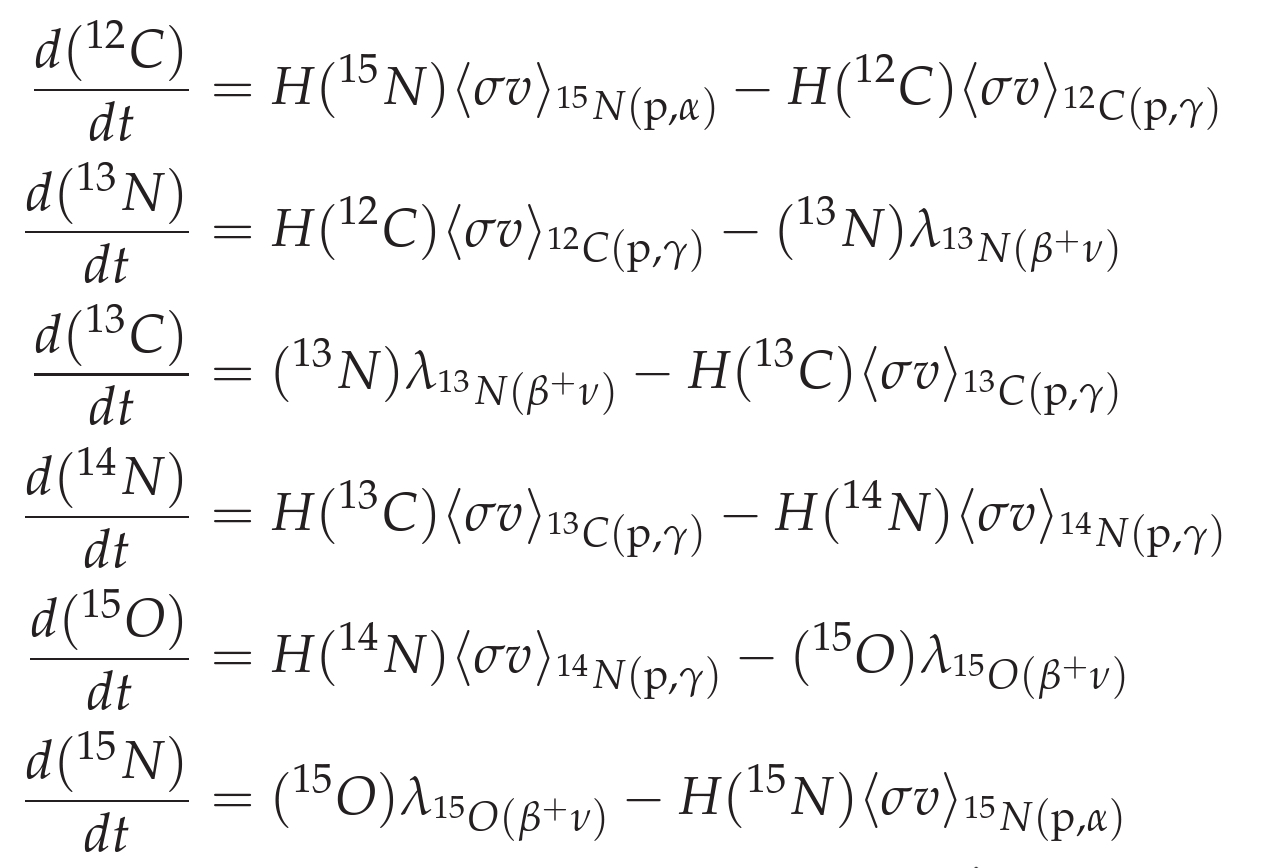
\includegraphics[trim={0cm 0cm 1cm 0cm},clip, keepaspectratio,height=0.28\textheight]{CNO1ab}
			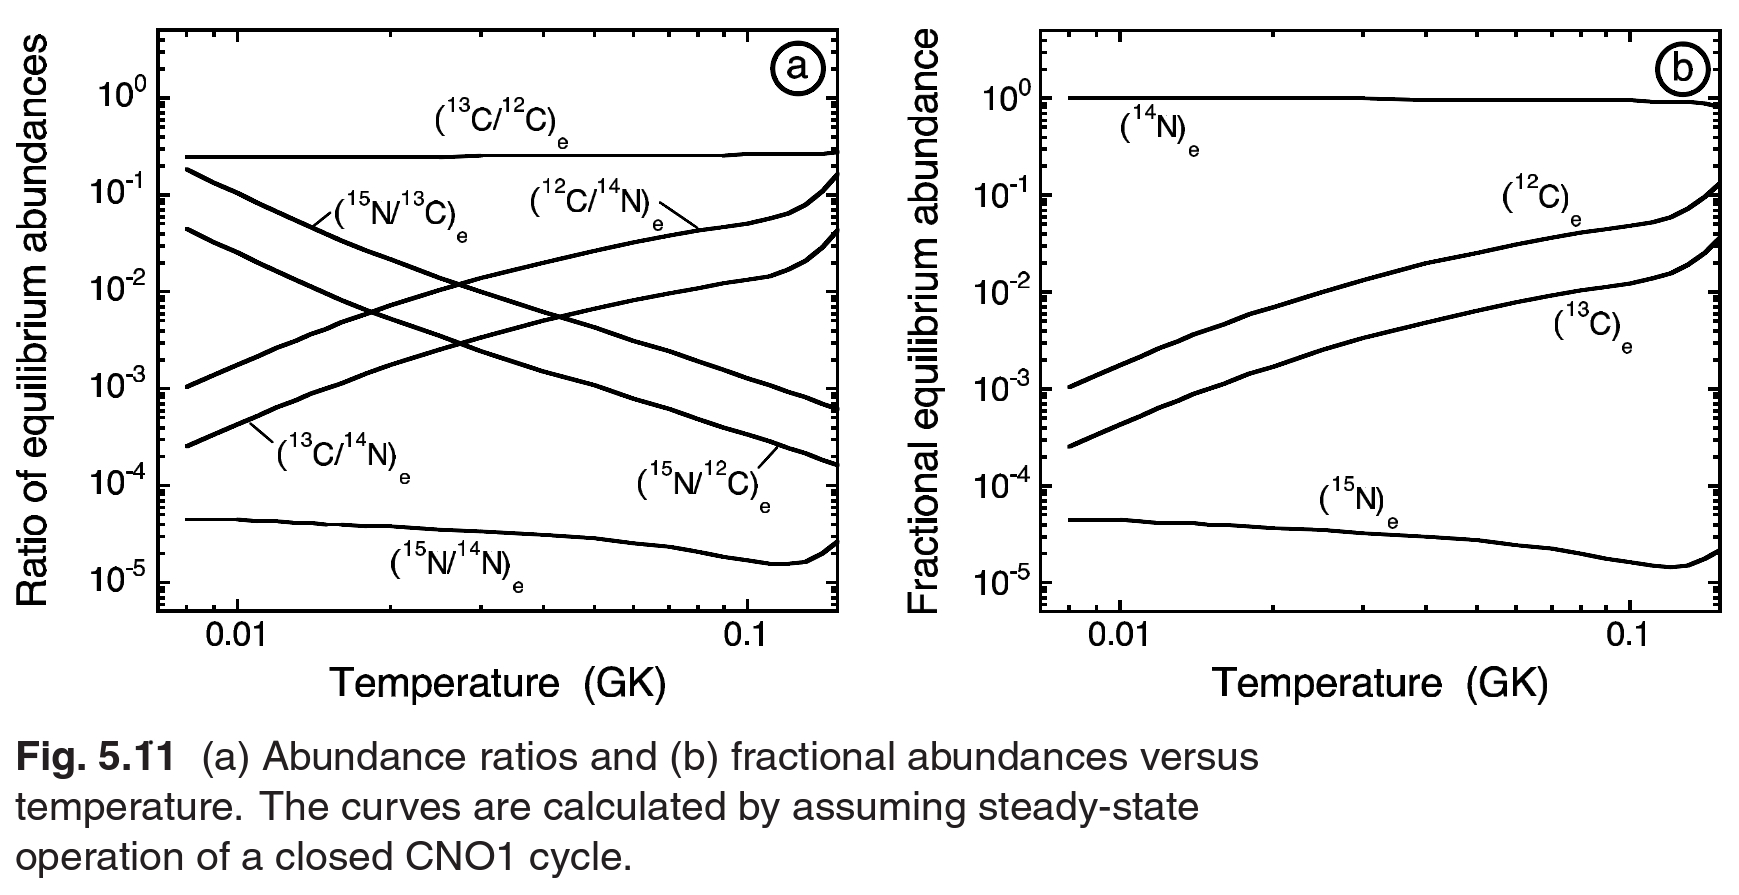
\includegraphics[trim={0cm 0cm 1cm 0cm},clip, keepaspectratio,height=0.28\textheight]{CNOXivsT}
		\end{figure}
	\end{column}
\end{columns}
\end{frame}

\begin{frame}{CNO1: energy production rate}

\begin{align*}
&\epsilon_{CNO1}=\sum_{i\to j}\epsilon_{i\to j}=\frac{1}{\rho}(Q_{i\to j}-\exv{E}_{\nu}^{i\to j})r_{i\to j}\\
&\rho\epsilon^e_{CNO1}=\SI{3.458}{\mega\ev}\frac{(^{12}C)_e}{\tau_p(^{12}C)}+\SI{7.551}{\mega\ev}\frac{(^{13}C)_e}{\tau_p(^{13}C)}+\SI{9.055}{\mega\ev}\frac{(^{14}N)_e}{\tau_p(^{14}N)}\\
&+\SI{4.966}{\mega\ev}\frac{(^{15}N)_e}{\tau_p(^{15}N)}\\
&\epsilon^e_{CNO1}\approx\SI{25.030}{\mega\ev}N_A\exv{\sigma v}_{^{14}N(p,\gamma)}(\sum_{CNO1}\frac{X_i}{M_i})\frac{X_H}{M_H}\rho N_A\si{\mega\ev\per\second\per\gram}\\
&\epsilon^e_{CNO1}=\epsilon^e_{CNO1}(T_0)(\frac{T}{T_0})\expy{16.7},\ T_0\approx\SI{25}{\mega\kelvin}\\
%%Q
&Q_{^{12}C(p,\gamma)^{13}N(\beta^+\nu)}-\exv{E}_{\nu}^{^{13}N(\beta^+\nu)}=(1.944+2.22-0.706)\si{\mega\ev}\\
&Q_{^{13}C(p,\gamma)}=\SI{7.551}{\mega\ev}\\
&Q_{^{14}N(p,\gamma)^{15}O(\beta^+\nu)}-\exv{E}_{\nu}^{^{15}O(\beta^+\nu)}=(7.297+2.754-0.996)\si{\mega\ev}\\
&Q_{^{15}N(p,\alpha)}=\SI{4.966}{\mega\ev}
\end{align*}

\end{frame}

\subsection{He-C-Ne-O-Si-Burning}\linkdest{epsilonheavy}

\begin{frame}{Combustion He}
\begin{columns}[T]
	\begin{column}{0.5\textwidth}
	\begin{itemize}
	\item Deps $M_*$ amd $Z$: hydrostatic He burning in massive star $\rho=\SIrange{e2}{e5}{\gram\per\cubic\cm}$, $T=\SIrange{0.1}{0.4}{\giga\kelvin}$
	\item Reactiona during He-buring
	\begin{align*}
&^4He(\alpha\alpha,\gamma)^{12}C\ Q=\SI{7274.7}{\kilo\ev}\\
&^{12}C(\alpha,\gamma)^{16}O\ Q=\SI{7161.9}{\kilo\ev}\\
&^{16}O(\alpha,\gamma)^{20}Ne\ Q=\SI{4729.8}{\kilo\ev}\\
&^{20}Ne(\alpha,\gamma)^{24}Mg\ Q=\SI{9316.6}{\kilo\ev}
	\end{align*}
\item Energy production by $3\alpha$:
\begin{align*}
&\epsilon_{3\alpha}=\frac{Q_{3\alpha}}{\rho}r_{3\alpha}=\frac{Q_{3\alpha}}{\rho}\frac{N_{\alpha}\lambda_{3\alpha}}{3}\\
&=\num{3.1771e14}\frac{\rho^2X_{\alpha}^3}{T_9^3}\exp{-\frac{4.4040}{T_9}}\si{\mega\ev\per\gram\per\second}\\
&\epsilon_{3\alpha}(T)=\epsilon_{3\alpha}(T_0)(\frac{T}{T_0})^{41}
\end{align*}
		\end{itemize}
	\end{column}
	\begin{column}{0.5\textwidth}
		\begin{figure}[!ht]
			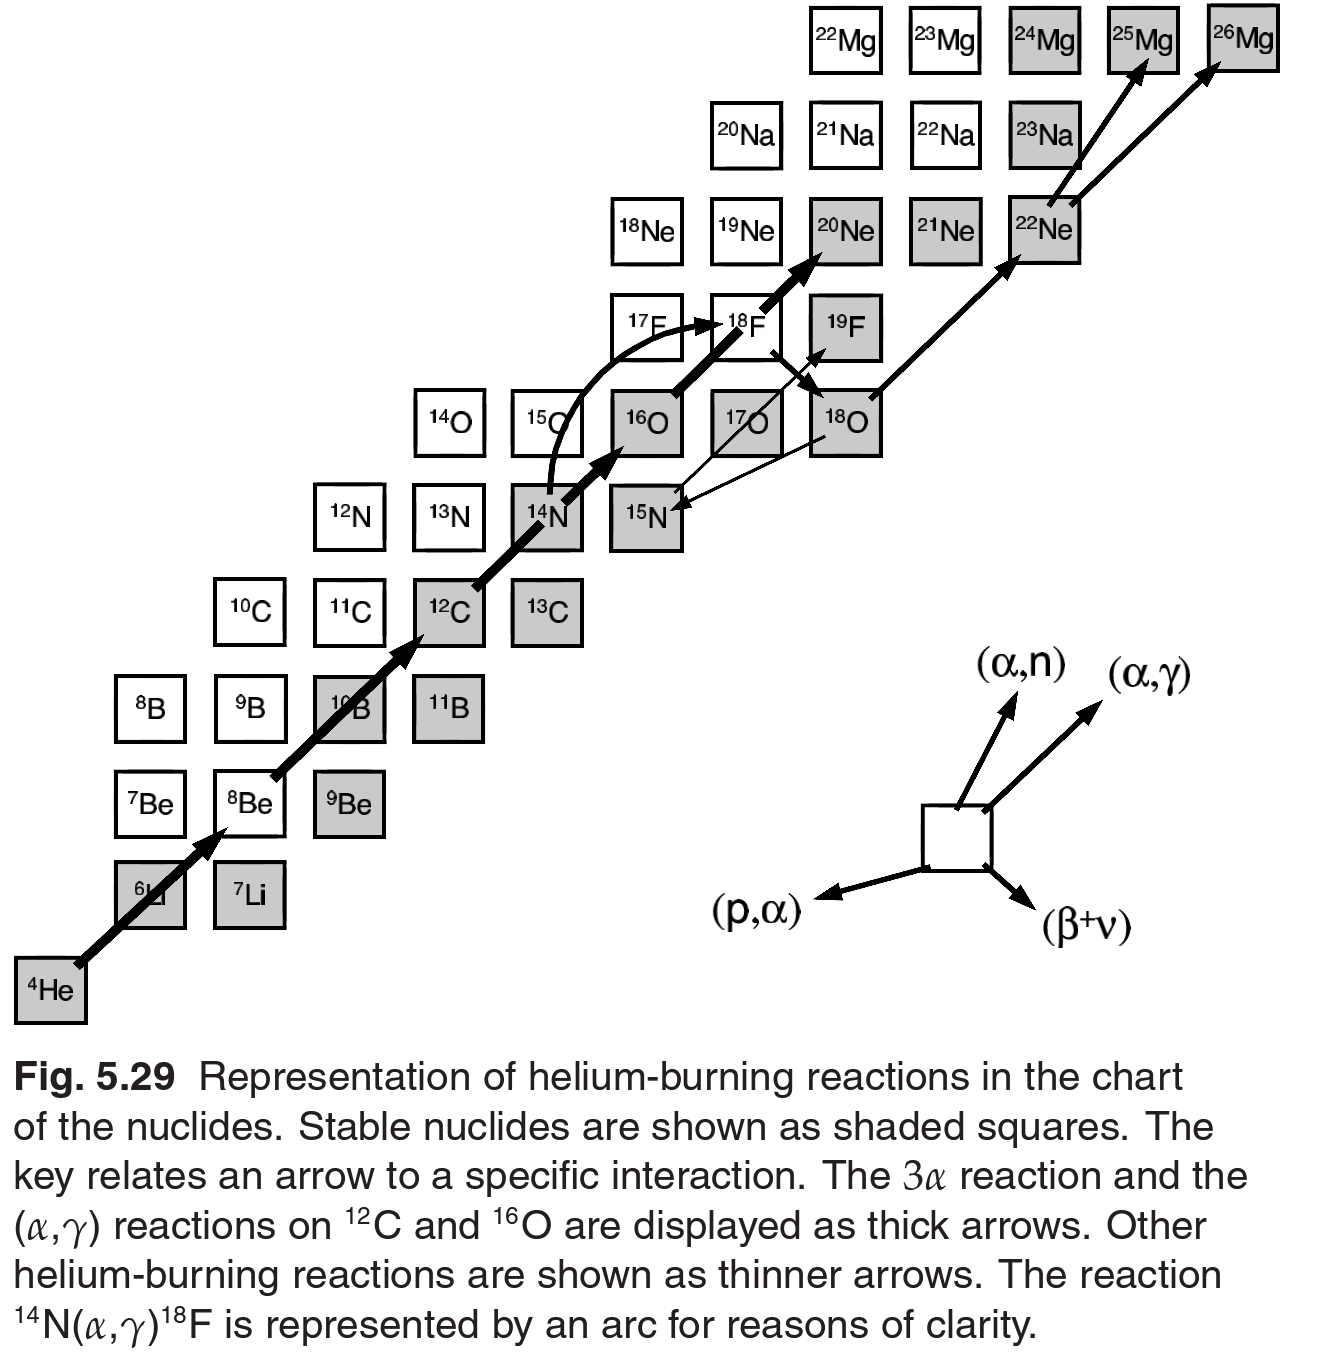
\includegraphics[trim={0cm 0cm 1cm 0cm},clip, keepaspectratio,height=0.28\textheight]{Heburningelems}
			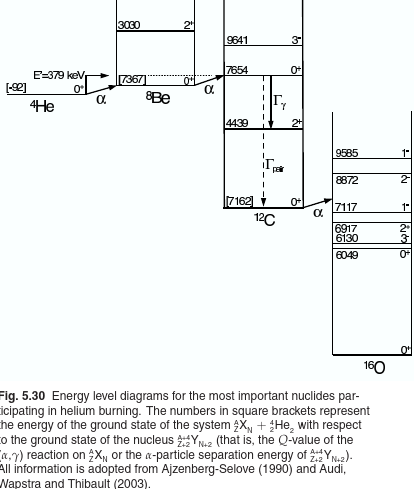
\includegraphics[trim={0cm 0cm 1cm 0cm},clip, keepaspectratio,height=0.28\textheight]{3alphalevels}
		\end{figure}
	\end{column}
\end{columns}
\end{frame}


\begin{frame}{Produzione nuclei fino al Fe56}
3$\alpha$: $He4+\alpha\to C12$, $C12+\alpha\to O16$
Produzione neutroni liberi
Fusione $C12$, fotodisintegrzione $Ne20$, fusione $O16$, fotodisintegrzione $Si28$, catture $\alpha$ su nuclei fino a produzione $Fe56$
\end{frame}

\begin{frame}{Cattura neutronica: processi r e s}
\todo{picchi r e s nella nella curva universale delle abbondanze}
\end{frame}

\begin{frame}{Nuclear burning efficiency}
\begin{equation*}
\epsilon_{ij}(\rho,T,X_i)=Q_{ij}\frac{n_in_j}{\rho(1+\delta_{ij})}\lambda_{ij}=\frac{1}{1+\delta_{ij}}Q_{ij}\frac{\rho N_A^2X_jX_k}{{A_iA_j}}\exv{\sigma v}_{ij}
\end{equation*}
dove $Q_{ij}$ \'e l'energia liberata per reazione tra nucleo di specie i e j e $\exv{\sigma v}_{ij}$ \'e il rate di reazione per coppia di particelle; $X_i$ indica la frazione in  massa della specie i
\begin{columns}[T]
	\begin{column}{0.5\textwidth}
		\begin{align*}
		&PP\ \exv{\sigma v}\propto T\expy{3.9}\ E_C=\SI{0.55}{\mega\ev}\\
		&P^{14}N\ \exv{\sigma v}\propto T\expy{20}\ E_C=\SI{2.27}{\mega\ev}\\
		&\alpha+^{12}C\ \exv{\sigma v}\propto T\expy{42}\ E_C=\SI{3.43}{\mega\ev}\\
		&^{16}O+^{16}O\ \exv{\sigma v}\propto T\expy{182}\ E_C=\SI{14.07}{\mega\ev}
		\end{align*}
	\end{column}
	\begin{column}{0.5\textwidth}
		\begin{align*}
		&E_C\approx Z_1Z_2\si{\mega\ev}
		\end{align*}
	\end{column}
\end{columns}
\end{frame}

\begin{frame}{Ripasso perdita neutrini}\linkdest{epsilonnu}
    
\end{frame}


\section{Ordini di grandezza e comportamento qualitativo}\linkdest{ormagandqual}

\begin{frame}{Core Contraction - Envelope Expansion}
    During evolution in HRD a star goes through different phases some of which involves core contraction-envelope expansion: since that happens in a variety of situation we need genaral principles:
    \begin{align*}
        &E=\exv{\Omega}+\exv{U}-\int_0^tL\,dt+\int_0^t\epsilon\,dt\tag{Tot. Energy, Av. over $t_{dyn}$}\\
        &\approx\exv{\Omega}+\exv{U}\approx\const{}\tag{$t<\tkh{}$}\\
        &\exv{\Omega}*2\exv{U}=0\tag{Virial}\\
        &\Rightarrow\Omega_c+\Omega_e\approx\const{}\\
        &\Omega\approx \frac{GM_c^2}{R_c}+\frac{GM_cM_e}{R_*}\tag{$M_e\ll M_c$ for UMS}\\
        &\Rightarrow \frac{R_*}{R_c}\approx-\frac{M_c}{M_e}(\frac{R_*}{R_c})^2\ll-1\tag{Assumption: $M_c\approx\const{},\ M_e\approx\const{}$}\\
        &\Rightarrow \frac{R_*}{R_c}\approx-\frac{M_c}{M_e}(\frac{R_*}{R_c})^2\approx-1\tag{LMS: $M_e>M_c$}
    \end{align*}
\end{frame}

\section{Politropic Models}\linkdest{poly}

\begin{frame}{Polytropic relation}
    \framesubtitle{$P=K\rho^{\gamma}=K\rho^{1+\frac{1}{n}}$}
Additional relation between T-P: ie $1^{st}$ law $\TDy{T}{Q}=\TDy{T}{U}+P\TDy{T}{V}=C=c_V+P(\TDy{T}{V})_P$ - ideal gas $c_P-c_V=\frac{R}{\mu}$: $\frac{dT}{T}+\frac{1}{n}\frac{dV}{V}=0$, $n=\frac{c_V-C}{c_P-c_V}$. \keyword{trasformazione politropa}: t. quasi-statica in  con $c=\TDy{Q}{T}$ (calore specifico) assegnato - K is free parameter.
Polytropic relation in stars:
\begin{itemize}
    \item Equation of state is of the form $P=K\rho^{\gamma}$, K fixed.
    \item EOS contains $T$ but exist additional relation between $P$ and $T$ yielding polytropic relation, $K$ is a free parameter
\end{itemize}
%$TV\expy{\gamma-1}=\const$, $PV\expy{\gamma}=\const$, $P\expy{1-\gamma}T\expy{\gamma}=\const$ ($0=dE-\frac{P}{\rho^2}d\rho$).
                \begin{itemize}
                    \item For completely degenerate gas EOS has polytropic form: NR($\gamma=\frac{5}{3}$, $n=\frac{3}{2}$), UR(\gamma=\frac{4}{3}$, $n=3$)
                    \item $\gamma=5/3, n=3/2$: NR deg
                    \item $\gamma=4/3, n=3$: R deg
                    \item $\gamma=1, n=\infty$: isothermal sphere
                    \item $\nad\approx\frac{2}{5}$: conv
                \end{itemize}
$w(0)=1$, $w'(0)\propto\TDy{r}{\phi}=|g|\to0$, $w(z\approx0)\approx1-\frac{1}{6}z^2+\ldots$
\end{frame}

\begin{frame}{Polytropic stellar model}
    \begin{columns}[T]
        \begin{column}{0.55\textwidth}
				\begin{align*}
                &\frac{1}{r^2}\TDof{r}(r^2\TDy{r}{\phi})=4\pi G\rho\tag{Poiss.}\\
                    &\TDy{r}{P}=-\TDy{r}{\phi}\rho\tag{HE}\\
                &\TDy{r}{\phi}=-\gamma K\rho\expy{\gamma-2}\TDy{r}{\rho}:\\
                &\rho=(\frac{-\phi}{(n+1)K})^n\tag{Const of integr.: $\phi=0$ at surf. $\rho=0$}\\
                &\TtwoDy{r}{\phi}+\frac{2}{r}\TDy{r}{\phi}=4\pi G(\frac{-\phi}{(n+1)K})^n\tag{Above into Poisson}\\
                &w(0)=1,\ \TDy{z}{w}=w'(0)=0\tag{At center: $z=0$}\\
                &\rho(r)=\rho_cw^n,\ P(r)=P_cw^{n+1},\ P_c=K\rho_c^{\gamma}
				\end{align*}
        \end{column}
        \begin{column}{0.45\textwidth}
			\begin{align*}
			&\rho=(\frac{-\phi}{(n+1)K})^n\tag{HE}\\
			&\TtwoDy{r}{\phi}+\frac{2}{r}\TDy{r}{\phi}=4\pi G(\frac{-\phi}{(n+1)K})^n\tag{Poiss}\\
            &z=Ar,\ w=\frac{\phi}{\phi_c}=(\frac{\rho}{\rho_c})\expy{1/n}\tag{new adim. vars: z,w}\\
			&A^2=\frac{4\pi G}{(n+1)^nK^n}(-\phi_c)\expy{n-1}=\frac{4\pi G}{(n+1)K}\rho_c\expy{\frac{n-1}{n}}\\
			&w=\frac{\phi}{\phi_c}=(\frac{\rho}{\rho_c})\expy{1/n}\ (\rho=\rho_cw^n)\\
			&\TtwoDy{z}{w}+\frac{2}{z}\TDy{z}{w}+w^n=0\\
			&\frac{1}{z^2}\TDof{z}(z^2\TDy{z}{w})+w^n=0\tag{Lane-Emden}
			\end{align*}
        \end{column}
    \end{columns}
    
\end{frame}

\begin{frame}{Equazione Lane-Emden: Properties of solutions $w(z)$}
    LE has regular singularity at $z=0$: expansion $w(z)=1+a_1z+a_2z^2+a_3z^3+\ldots$, with $a_1=w'(0)$, $2a_2=w''(0)$, \ldots{}; since grav. accel. $|\vec{g}|=\TDy{r}{\phi}\approx\TDy{z}{w}$ must vanish at center: $a_1=0$. Inserting expansion near $z=0$ into LE eq. and comparing coeffs. we find $w(z)=1-\frac{1}{6}z^2+\frac{n}{120}z^4+\ldots$ (excluding $n=\infty$): $w(z)$ has max. at $z=0$.
    Surface where $w(z_n)=0$ and $\rho=0$ ($\frac{r}{z}=\frac{1}{A}=\frac{R}{z_n}$): $z_0=\sqrt{6},\ z_1=\pi,\ldots,z_{5}=\infty$ (\xaumenta{n},\xaumenta{z_n}) also central concentration $\frac{\rho_c}{\bar{\rho}}$ increases. For non-complete polytrope, ie convective envelope, behaviour at center may be unimportant.
\end{frame}

\begin{frame}{Polytropic star model: given $n<5, M, R$}
\begin{block}{Possible if K not fixed by eos}
    \begin{columns}[T]
        \begin{column}{0.6\textwidth}
    \begin{align*}
&m(r)=\int_0^r4\pi\rho r^2\,dr=4\pi\rho_c\int_0^rw^nr^2\,dr=4\pi\rho_c\frac{r^3}{z^3}\int_0^zw^nz^2\,dz\\
&=4\pi\rho_cr^3(-\frac{1}{z}\TDy{z}{w}),\ M=4\pi\rho_cR^3(-\frac{1}{z}\TDy{z}{w})_{z=z_n}\\
&\frac{\exv{\rho}}{\rho_c}=[-\frac{3}{z}\TDy{z}{w}]_{z_n}\\
&\rho=\rho_cw^n(z),\ P=K(A,\rho_c)\rho^{\frac{n+1}{n}}
\end{align*}
        \end{column}
        \begin{column}{0.4\textwidth}
            \begin{align*}
            &w=\frac{\phi}{\phi_c}=(\frac{\rho}{\rho_c})^n\\
            &\rho(r)=\rho_cw^n,\ \TDof{z}(z^2\TDy{z}{w})=-z^2w^n\\
            &\frac{r}{z}=\frac{1}{A}=\frac{R}{z_n}
            \end{align*}
        \end{column}
    \end{columns}
    If n is given we solve LE: $w(z)$, $w'(z)$, $z_n$, $-\frac{z_n}{3\TDy{z}{w}|_{z_n}}$. Using $M,R$ we get $\bar{\rho}$ then $\rho_c$. On the other hand we know $A=\frac{z}{r}=\frac{z_n}{R}$: we get $K$ inverting definition of A. So $\rho(r)=\rho_cw^n(z)$, $P(r)=K\rho^{\frac{n+q}{n}}=K\rho_c^{\frac{n+1}{n}}w^{n+1}$
\end{block}
\begin{columns}[T]
\begin{column}{0.6\textwidth}
\begin{block}{Radiative pressure and $n=3$}
	\begin{align*}
    &n=3, P\propto\rho T: T\propto P^{\frac{1}{4}}\\
    &P=\frac{R\rho}{\mu}+\frac{a}{3}T^4=\frac{R}{\mu\beta}\rho T\\
    &\beta=\frac{P_{gas}}{P},\ 1-\beta=\frac{P_r}{P}=\frac{aT^4}{3P}\\
    &\Rightarrow P=(\frac{3R^4}{a\mu^4})^{\frac{1}{3}}(\frac{1-\beta}{\beta^4})^{\frac{1}{3}}\rho^{\frac{4}{3}}
	\end{align*}
Eddington: $\frac{\kappa l}{m}$ const throughout star then $\beta=\const{}$, then polytropic rel.
\end{block}
\end{column}
\begin{column}{0.40\textwidth}
    \begin{block}{Sun}
        \begin{align*}
            &n=3,\,M=\SI{1.989e33}{\gram}\\
            &R=\SI{6.96e10}{\cm}, z_3=6.897\\
            &\frac{\rho_c}{\bar{\rho}}=54.18: \bar{\rho}=\SI{1.41}{\gram\per\cubic\cm}\\
            &\rho_c=\SI{76.39}{\gram\per\cubic\cm},A=\frac{z_3}{R}=\num{9.91e-11}\\
            &K=\num{3.85e14},\,P_c=\SI{1.24e17}{\dyn\per\square\cm}
        \end{align*}
    \end{block}
\end{column}
\end{columns}
\end{frame}

\begin{frame}{Isothermal sphere: $\gamma=1, n\to\infty$}
    \begin{itemize}
        \item $K=\frac{RT}{\mu}$ free param
        \item hydrostatic condition for polytropes gives $\frac{\phi}{-K}=\ln{\rho}-\ln{\rho_c}$ so $\rho=\rho_c\exp{-\frac{\phi}{K}}$.
        \item Poiss. eq $\TtwoDy{r}{\phi}+\frac{2}{r}\TDy{r}{\phi}=4\pi G\rho_c\exp{-\frac{\phi}{K}}$
        \item Adimensional Variables w,z ($z=Ar$, $A^2=\frac{4\pi G\rho_c}{K}$, $\phi=Kw$): $\TtwoDy{z}{w}+\frac{2}{z}\TDy{z}{w}=\exp{-w}$ isothermal LE equation with central condition $w(0)=w'(0)=0$.
    \end{itemize}
    \end{frame}

\begin{frame}{Fixed K.: NR deg. electron gas. WD, $M_{ch}$}
\begin{block}{NR degenerate \Pelectron gas}
    EOS for NR \Pelectron degnerate gas: $n=\frac{3}{2}$, $K=\frac{1}{20}(\frac{3}{\pi})^{\frac{3}{2}}\frac{h^2}{m_e}\frac{1}{(\mu_em_p)^{\frac{5}{3}}}$.
\end{block}
\begin{block}{WD model: index n, given $\rho_c$ - 1D-manifold}
    \begin{columns}[T]
        \begin{column}{0.5\textwidth}
            \begin{itemize}
                \item $w(z)$, $w'(z)$ given by integration of LE equation
                \item Given $\rho_c$ the poly model gives $\rho=\rho_cw^n$ as function of z, relation between r,z is $(\frac{r}{z})^2=\frac{1}{A^2}=\frac{1}{4\pi G}(n+1)K\rho_c\expy{\frac{1-n}{n}}$, $R=\frac{z_n}{A}\propto\rho_c^{\frac{1-n}{2n}}$
                \item $R\propto\rho_c\expy{\frac{1-n}{2n}}$: as long as $n>1$, R decreases as $\rho_c$ increases.
            \end{itemize}
        \end{column}
        \begin{column}{0.5\textwidth}
            \begin{itemize}
                \item $M\propto\rho_cR^3$: $M=C_1\rho_c\expy{\frac{3-n}{2n}}$, $C_1=4\pi(-\frac{w'}{z})_{z_n}z_n^3(\frac{n+1}{4\pi G})\expy{\frac{3}{2}}K\expy{\frac{3}{2}}$
                \item Mass-radius relation: $R\propto M\expy{\frac{1-n}{3-n}}$
            \end{itemize}
        \end{column}
    \end{columns}
\end{block}
\begin{block}{$M_{Ch}$: fitting relativistic $n=3$ with NR $n=\frac{3}{2}$}
    Relativistic core for $\rho_c>\SI{e6}{\gram\per\cubic\cm}$, expecting model approach state where is fully relativistic, $n=3$, $M=C_1=4\pi(-\frac{w'}{z})_{z_n}z_n^3(\frac{n+1}{4\pi G})^{\frac{3}{2}}K^{\frac{3}{2}}$: $M_{ch}=\frac{5.836}{\mu_e^2}\msun{}$; when all H is transformed into He, C, O: $\mu_e=2$, $M_{Ch}=1.46\msun{}$. So our series of models with increasing central density tend to finite mass and approach zero radius for $\rho_c\to\infty$.
\end{block}
\end{frame}

\begin{frame}{Energy in poly}
Energia gravitazionale:
\begin{align*}
&E_g=-G\int_0^M\frac{m}{r}\,dm=\overbrace{-\frac{1}{2}\frac{GM^2}{R}}^{\int m\,dm}\overbrace{-\frac{1}{2}G\int_0^R \frac{m^2}{r^2}\,dr}^{dm=4\pi r^2\,dr, \TDof{m}=\frac{1}{4\pi r^2\rho}\TDof{r}}\\
&=-\frac{1}{2}\frac{GM^2}{R}-\frac{1}{2}\int_0^R\TDy{r}{\phi}m\,dr=-\frac{1}{2}\frac{GM^2}{R}\overbrace{+\frac{1}{2}\int_0^M\phi\,dm}^{m=0: m\phi=0,\ \phi=0: m\phi=0}\tag{$\TDy{r}{\phi}=\frac{Gm}{r^2}$}\\
&\phi=-\frac{K\gamma}{\gamma-1}\rho^{\gamma-1}=-\frac{\gamma}{\gamma-1}\frac{P}{\rho}\tag{poly}\\
&E_g=-\frac{1}{2}\frac{GM^2}{R}-\frac{1}{2}\frac{\gamma}{\gamma-1}\int_0^M \frac{P}{\rho}\,dm=-\frac{1}{2}\frac{GM^2}{R}+\frac{1}{6}(n+1)E_g: E_g=-\frac{3}{5-n}\frac{GM^2}{R}\tag{$E_g=-3\int_0^M\frac{P}{\rho}\, dm$}
\end{align*}
Energia interna $E_i$ della stella - $u$ per unit mass:
\begin{align*}
&\frac{P}{\rho}=\frac{R}{\mu}T=\frac{c_P-c_V}{\mu}T=(\gamma-1)c_VT(\xrightarrow{\text{m.g.:}\gamma=\frac{5}{3}}\frac{2}{3}u):\ \zeta=\frac{3P}{\rho u}\xrightarrow{i.g.}3(\gamma_{Ad}-1)\tag{virial for general EOS: $\zeta E_i+E_g=0$}\\
&\zeta\,du=3\frac{dP}{\rho}-3\frac{P}{\rho^2}\,d\rho\to 3\frac{\rho}{P}\TDy{\rho}{P}-3=3(\gamma_{Ad}-1)\tag{Adiabatic changes, First: $du=\frac{P}{\rho^2}\,d\rho$, $\gamma_{Ad}=\frac{\rho}{P}\TDy{\rho}{P}$}\\
&E_i=-\frac{1}{\zeta}E_g=\frac{3}{\zeta(5-n)}\frac{GM^2}{R},\ W=E_i+E_g=\frac{3}{5-n}(\frac{1}{\zeta}-1)\frac{GM^2}{R}
\end{align*}
\end{frame}

\section{Homologous Relations}\linkdest{homology}

\begin{frame}{Homologous Stars}
    Comparing two models for $M,R$ and $M',R'$ are homologous if h. mass shell, $\frac{m}{M}=\frac{m'}{M'}$, are at h. points, $\frac{r}{R}=\frac{r'}{R'}$.
    \begin{columns}[T]
        \begin{column}{0.55\textwidth}
            \begin{align*}
                &\xi=\frac{m}{M}=\frac{m'}{M'}: \frac{r(\xi)}{r'{\xi}}=\frac{R}{R'}\\
                &\begin{array}{l}
                \frac{r}{r'}=z=\frac{R}{R'},\frac{P}{P'}=p=\frac{P_c}{P_c'}\\
                \frac{T}{T'}=t=\frac{T_c}{T_c'},\frac{l}{l'}=s=\frac{L}{L'}
            \end{array}\tag{Ansaz}\\
            &\begin{array}{l}
                \TDy{\xi}{r}=c_1 \frac{M}{r^2\rho},c_1=\frac{1}{4\pi}\\
                \TDy{\xi}{P}=c_2 \frac{\xi M^2}{r^4},c_2=-\frac{G}{4\pi}\\
                \TDy{\xi}{l}=\epsilon M,\TDy{\xi}{T}=c_4 \frac{\kappa lM}{r^4T^3},c_4=-\frac{3}{64\pi^2ac}
            \end{array}\\
            &\begin{array}{l}
                \TDy{\xi}{r'}=c_1 \frac{M'}{r'^2\rho'}[\frac{x}{z^3d}],\TDy{\xi}{P'}=c_2 \frac{\xi M'^2}{r'^4}[\frac{x^2}{z^4p}]\\
                \TDy{\xi}{l'}=\epsilon'M'[\frac{ex}{s}],\TDy{\xi}{T'}=c_4 \frac{\kappa'l'M'}{r'^4T'^3}[\frac{ksx}{z^4t^4}]
            \end{array}\\
            &\frac{x}{z^3d}=1, \frac{x^2}{z^4p}=1, \frac{ex}{s}=1, \frac{ksx}{z^4t^4}=1\\
            &\begin{psmallmatrix}
                -3&-\alpha&\delta&0\\
                -4&-1&0&0\\
                0&\lambda\alpha&(\nu-\lambda\delta)&-1\\
                -4&a&(b-4)&1\\
            \end{psmallmatrix}
            \begin{psmallmatrix}
                z_1\\p_1\\t_1\\s_1\\
            \end{psmallmatrix}=\begin{psmallmatrix}
                -1\\-2\\-1\\-1\\
            \end{psmallmatrix}\tag{x}\\
            &\begin{psmallmatrix}\setlength\arraycolsep{-10pt}
                -3&-\alpha&\delta&0\\
                -4&-1&0&0\\
                0&\lambda\alpha&(\nu-\lambda\delta)&-1\\
                -4&a&(b-4)&1\\
            \end{psmallmatrix}
            \begin{psmallmatrix}
                z_2\\p_2\\t_2\\s_2\\
            \end{psmallmatrix}=\begin{psmallmatrix}
               \phi\\0\\-\lambda\phi\\0\\
            \end{psmallmatrix}\tag{y}
            \end{align*}
        \end{column}
        \begin{column}{0.45\textwidth}
            \begin{itemize}
                \item All h. mass shell are shifted by factor $\frac{R}{R'}$: any polytropes of same index are h.
                \item Ansaz: for h. mass values ratios $z$, $p$, $t$, $s$ have same values for all $\xi$
                \item Two stars are hydrostatic/thermal equilibrium, energy transport is radiative.
                \item z,p,t,s are indep. of $\xi$, $\xi$ contains contains tot. mass as scaling factor. Def.: $x=\frac{M}{M'}$, $y=\frac{\mu}{\mu'}$; $d=\frac{\rho}{\rho'}$, $e=\frac{\epsilon}{\epsilon'}$, $k=\frac{\kappa}{\kappa'}$ for ratios of material function at h. points.
                \item Since $r'$, $P'$, $T'$, $l'$ must fulfill same basic equations as $r$, $P$, $T$, $l$ $[]$ must be equal to one
                \item Repres. material functions by power law: $\rho\propto P^{\alpha}T^{-\delta}\mu^{\phi}$, $\epsilon\propto\rho^{\lambda}T^{\nu}$, $\kappa\propto P^aT^b$: $d=p^{\alpha}t^{-\delta}y^{\phi}$, $e=p^{\lambda\alpha}t^{\nu-\lambda\delta}y^{\lambda\phi}$, $k=p^at^b$.
                \item We will try to represent the ratios z,p,t,s in terms of x,y: $z=x^{z_1}y^{z_2}$, $p=x^{p_1}y^{p_2}$, $t=x^{t_1}y^{t_2}$, $s=x^{s_1}y^{s_2}$.
                \item Substituting the above into conditions for $[]$s we have the conditions that exponents of x and y must sum to 0.
            \end{itemize}
        \end{column}
    \end{columns}
\end{frame}

\begin{frame}{Solution for exponents of x,y and applications to simple material functions}
    \begin{align*}
            &z_1=\frac{1}{2}(1+A),p_1=-2A,t_1=\frac{1}{2\delta}[1+(3-4\alpha)A],s_1=1+\frac{4-b}{2\delta}+[2+2a+\frac{3-4\alpha}{2\delta}(4-b)]A\\
            &z_2=\phi B,p_2=-4\phi B,t_2=\frac{\phi}{\delta}[1+(3-4\alpha)B],s_2=\frac{\phi}{\delta}(4-b)+\phi[4+4a+\frac{3-4\alpha}{\delta}(4-b)]B\\
            &A=\invers{[\frac{4\delta(1+a+\lambda a)}{\nu+b-4-\lambda\delta}+4\alpha-3]},B=A\invers{(1-\frac{\lambda\delta}{\nu+b-4})}\\
            &\frac{x}{z^3d}=1\Rightarrow \frac{\rho}{\rho'}=\frac{M/M'}{(R/R')^3},\frac{x^2}{z^4p}=1\Rightarrow \frac{P}{P'}=\frac{(M/M')^2}{(R/R')^4}\tag{H. points: $\frac{r}{r'}=z$, $\xi=\frac{m}{M}=\frac{m'}{M'}$, $\frac{r(\xi)}{r'(\xi)}=\frac{R}{R'}$}
    \end{align*}
For all h. points density changes as mean density while $P\propto M^2R^{-4}$.
\begin{columns}[T]
    \begin{column}{0.3\textwidth}
        \begin{block}{$\delta=0$: polytropic}
            \begin{align*}
                &n=\frac{\alpha}{1-\alpha}\\
                &A=\invers{(4\alpha-1)}\\
                &z_1=\frac{2\alpha-1}{4\alpha-3}\\
                &R\propto M^{z_1}\tag{MR-rel, $y=1$}\\
                &\alpha=\frac{3}{5}:\\
                &z_1=-\frac{1}{3}\tag{NR \Pelectron gas}
            \end{align*}
        \end{block}
    \end{column}
    \begin{column}{0.38\textwidth}
        \begin{block}{Ideal gas, const $\kappa$: $\alpha=\delta=\phi=1$, $a=b=0$}
            \begin{align*}
                &z_1=\frac{\nu+\lambda-2}{\nu+3\lambda},z_2=\frac{\nu-4}{\nu+3\lambda}\\
                &p_1=2-4z_1,p_2=-4z_2\\
                &t_1=1-z_1,t_2=1-z_2\\
                &s_1=3,s_2=4\\
                &\Rightarrow \frac{L}{L'}=(\frac{M}{M'})^3(\frac{\mu}{\mu'})^4\tag{$ML$,$L\mu$ rel}\\
                &\frac{R}{R'}=(\frac{M}{M'})^{z_1}(\frac{\mu}{\mu'})^{z_2}\tag{$z_1\in\numrange{0.4}{0.8}$}
            \end{align*}

        \end{block}
    \end{column}
    \begin{column}{0.32\textwidth}
        \begin{block}{Role EOS}
            Approx if material function don't contain only products:
            \begin{align*}
                &\rho=(\mu\beta)\frac{P}{T},\beta=\frac{P_g}{P}=1-\frac{P_r}{P}\\
                &R\propto\beta^{z_2},P\propto\beta^{p_2}\\
                &T\propto\beta^{t_2},L\propto\beta^{s_2}\tag{$\beta$ det. by $P,T$}\\
                &1-\beta=\frac{P_r}{P}\propto \frac{T^4}{P}\propto\frac{M^{4t_1}}{M^{p_1}}\frac{\beta^{4t_2}}{\beta^{p_2}}
            \end{align*}
        \end{block}
    \end{column}
\end{columns}

\end{frame}

\begin{frame}{Homologous contraction (poly index n)}
    Consecutive models are h. to each others, ie contraction of polytrope that doesn't change polytropic index; $z\propto\frac{r}{R}$ dim-less radius var: LE eqs gives $m(z)$ so mass elements at homologous points, mass elements ($\xi=\frac{m}{M}=\const{}$) remains at h. points, since their value of z do not change in time.
\begin{align*}
&r'=r+\dot{r}\Delta t\Rightarrow\frac{r}{r'}=1+\frac{\dot{r}}{r}\Delta t\\
&\frac{r'}{r}=\frac{R'}{R}=\const{}\Rightarrow\frac{\dot{r}}{r}=\frac{\dot{R}}{R}=\const{}\ (\PDof{m}\PDy{t}{\ln{r}})=0\\
&\PDof{t}(\frac{1}{r}\PDy{m}{r})=0=\PDof{t}(\frac{1}{4\pi r^3\rho})\Rightarrow\frac{\dot{\rho}}{\rho}=-3\frac{\dot{r}}{r}\\
&P=\int_m^M\frac{Gm}{4\pi r^4}\,dm:\ \dot{P}=\int_m^M\PDof{t}(\frac{1}{r^4})\frac{Gm}{4\pi}\tag{HE}\\
&\rho\propto P^{\alpha}T^{-\delta}\Rightarrow\frac{\dot{\rho}}{\rho}=\alpha\frac{\dot{P}}{P}-\delta\frac{\dot{T}}{T}\tag{EOS}\\
&\frac{\dot{T}}{T}=-\frac{4\alpha-3}{\delta}\frac{\dot{r}}{r}\\
&\epsilon_g=c_PT(\nad\frac{\dot{P}}{P}-\frac{\dot{T}}{T})=c_PT[-4\nad+\frac{4\alpha-3}{\delta}]\frac{\dot{R}}{R}\\
&\to-\frac{3}{5}c_PT\frac{\dot{R}}{R}\tag{ideal mono $\nad=\frac{2}{5}$, $\alpha=\delta=1$}\\
&\frac{1-\beta}{\beta^4}\propto M^2\tag{replacing expression for exponent}
\end{align*}
\end{frame}


\section{Stellar Atmosphere}


\section{Metodi per integrazione equazioni di struttura e raccordo con modelli dell'atmosfera stellare}\linkdest{stellarsolve}

\subsection{4 Structure ODE with boundary conditions}\linkdest{fourODE}

\begin{frame}{Equazioni struttura di equilibrio}
\begin{align*}
&\TDy{m}{r}=\frac{1}{4\pi r^2\rho}\\
&\TDy{m}{P}=-\frac{Gm}{4\pi r^4}\overbrace{[-\frac{1}{4\pi r^2}\PtwoDy{t}{r}]}^{\tau_{hyd}}\\
&\TDy{m}{T}=-\nabla\frac{T}{p}\frac{Gm}{4\pi r^4}\\
&\TDy{m}{L}=\epsilon-\epsilon_{\nu} \underbrace{-c_P[\TDy{t}{T}-\nad\frac{T}{P}\TDy{t}{P}]}_{-c_P\PDy{t}{T}+\frac{\delta}{\rho}\PDy{t}{P}: \tkh}\\
&\TDy{t}{X_s}\frac{1}{A_s}=\sum_{production}\rho^{n_h+n_k-1}n_p\frac{X_h^{n_h}X_k^{n_k}}{A_h^{n_h}A_k^{n_k}}\frac{\exv{\sigma v}_{hk}}{m_H^{n_h+n_k-1}n_h!n_k!}\\
&-\sum_{distruction}\rho^{n_d+n_j-1}n_d\frac{X_s^{n_d}X_j^{n_j}}{A_s^{n_d}A_j^{n_j}}\frac{\exv{\sigma v}_{sj}}{m_H^{n_d+n_j-1}n_d!n_j!}
\end{align*}
\end{frame}

\begin{frame}{Condizioni al bordo: espansione condizioni al centro ($m\to0$)}
\begin{itemize}
\item Le 4+I equazioni determinano $r$, $P$, $T$, $L$, $X_s$ specificata la massa e composizione iniziale (omogenea)
\item $\tau_n\gg\tkh\gg\tau_{dyn}$: solve 4 structure equations at time t - do time step $\Delta t$ and determine new composition - solve structure at $t+\Delta t$ with new composition
\item Solution of 4 structure equations require 4 boundary condition: 2 at surface (atmospere model without diffusion approx, PP geometry), parametri $\rho_c,T_c$; 2 at center (via Taylor expansion for $m=m'$)
\end{itemize}
\begin{columns}[T]
\begin{column}{0.65\textwidth}
\begin{align*}
    &d(r^3)=\frac{3}{4\pi\rho}\,dm\tag{to be integrated for $\rho=\rho_c$:}\\
&r=(\frac{3}{4\pi\rho_c})\expy{1/3}{m'}\expy{1/3}\\
&P=P_c-\frac{3G}{8\pi}(\frac{4\pi\rho_c}{3})\expy{4/3}{m'}\expy{2/3}\tag{r into HE and integrate}\\
&L=(\epsilon_n-\epsilon_{\nu}+\epsilon_g)_cm'\\
&\nabla=\TlnDy{P}{T},\ \nad{}=\frac{P\delta}{T\rho c_P},\ \nrad{}=\frac{3}{16\pi acG}\frac{\kappa lP}{mT^4}\\
&\TDy{m}{T}=-\frac{3}{64\pi^2ac}\frac{\kappa l}{r^4T^3}\tag{rad}\\
&T^4=T_c^4-\frac{1}{2ac}(\frac{3}{4\pi})\expy{2/3}\kappa_c\epsilon_c\rho_c\expy{4/3}{m'}\expy{2/3}\tag{rad}\\
&\ln{T}=\ln{T_c}-(\frac{\pi}{6})\expy{1/3}G\frac{{\nad}_c\rho_c\expy{4/3}}{P_c}{m'}\expy{2/3}\tag{con}
\end{align*}
\end{column}
\begin{column}{0.35\textwidth}
At surface $m=M$, $L=L_s$, atmospheric model for $P$, $T$ - atmosphere defined by $g=\frac{GM}{R^2}$, $T_e$, composition: provides $P_s$ at $\tau$ where diffusion approx. starts to be valid
\end{column}
\end{columns}
\end{frame}

\begin{frame}[fragile]{Al centro: 1-order expansion of structure equations as $m\to0$}
	\begin{align*}
	&d(r^3)=\frac{3}{4\pi\rho}:\ r=(\frac{3}{4\pi\rho_c})^{1/3}m^{1/3}\\
	&l=(\epsilon_n-\epsilon_{\nu}+\epsilon_g)_cm\\
	&\TDy{m}{P}=-\frac{GM}{4\pi r^4}=-\frac{G}{4\pi}(\frac{4\pi\rho_c}{3})^{4/3}m^{-1/3}\\
	&P-P_c=-\frac{3G}{8\pi}(\frac{4\pi\rho_c}{3})^{4/3}m^{2/3}\\
	&\TDy{r}{P}\propto\frac{m}{r^2}\to0\\
	&\TDy{m}{T}=-\frac{T}{P}\frac{Gm}{4\pi r^4}\nabla:\\
	&T^4-T_c^4=-\frac{1}{2ac}(\frac{3}{4\pi})^{2/3}\kappa_c(\epsilon_n-\epsilon_{\nu}+\epsilon_g)_c\rho_c^{4/3}m^{2/3}\tag{Radiative}\\
	&\log{T}-\log{T_c}=-(\frac{\pi}{6})^{1/3}G\frac{\nad{}_{,c}\rho_c^{4/3}}{P_c}m^{2/3}\tag{convective}
	\end{align*}
\end{frame}

\begin{frame}{Condizione alla superficie: fitting mass}
    Fotosfera: regione di emissione della radiazione $\tau=\int_R^{\infty}\kappa\rho\,dr=\exv{\kappa}\int_R^{\infty}\rho\,dr=\frac{2}{3}$. HE: pressure is given by weight of matter above $P(R)=\frac{2}{3}\frac{GM}{R^2}\frac{1}{\exv{\kappa}}$; $L=4\pi R^2\sigma T_e^4$: these photospheric condition represent two relations between surface values ($m\to M$) of functions $P, T, r, l$ but at photosphere photon mean free path is large so we need to fit interior solution to atmosphere solution.
    Fitting mass $m_F$: where interior equations still valid, $l\approx L$, $m\approx M$, $M-m_F\approx 0$: the smaller the lesser energy can be stored/released in this layer, so we can have thermally adjusted outer solution with $l\approx L$.
    Model of stellar atmosphere for given M, $X_i(m)$: two parameter solution $(R,T_e)$ that can be extended down to $m_F$ where we find  $l=l_F^{ex}=L$, $P=P_F^{ex}$, $T=T_F^{ex}$, $r=r_F^{ex}$ integrated down to $m_F$ to be matched with interior solutions.
    $r_F^{ex}=r_F^{in},\ P_F^{ex}=P_F^{in},\ T_F^{ex}=T_F^{in},\ l_F^{ex}=l_F^{in}$: 4 equations for 4 DOF, $T_c$, $P_c$, $T_e$, $R$, and we can invert $r_F^{ex}(R,L)$ obtaining $R=R(r_F^{ex},L)$ that inserted in function $P_F^{ex}$, $T_F^{ex}$:
\begin{columns}[T]
\begin{column}{0.5\textwidth}
\begin{align*} 
&P_F^{ex}(R(r_F^{ex},L),L)=\pi(r_F^{ex},L)\\
&T_F^{ex}(R(r_F^{ex},L),L)=\theta(r_F^{ex},L)
\end{align*}
\end{column}
\begin{column}{0.5\textwidth}
    If these are fullfilles there's always an outer solution that matches interior solution.
\begin{align*}
&P_F^{in}=\pi(r_F^{in},L)\\
&T_F^{in}=\theta(r_F^{in},L)
\end{align*}
\end{column}
\end{columns}

\end{frame}

\begin{frame}{Deps of interior solution on surface condition}
    m,l approx const in envelope, take P as indep. var: radiative envelope $\PDy{P}{T}=\frac{3}{64\pi\sigma G}\frac{\kappa l}{T^3m}$, $\kappa=\kappa_0P^aT^b$ con $a>0(=1)$, $b<0(=-4.5)$ resulting in $\frac{T^{3-b}}{P^a}\PDy{P}{T}=\frac{3\kappa_0}{64\pi\sigma G}\frac{l}{m}$ and taking $l\approx L$, $m\approx M$, the solution is $T^{4-b}=B(P^{1+a}+C)$ (''adiabat''). Fixing $a=1$, $b=-4.5$, Kramers opacity for BF, FF absorption:

Radiative Envelope
\begin{itemize}
	\item $C=0\Rightarrow \nabla=\TDly{P}{T}\approx0.235<\nad=\frac{2}{5}$ ($P=0|_{T=0}$)
	\item $C>0: \nabla<0.235$ (envelope sol. for $T_e>\SI{e4}{\kelvin}$):  $P^2\ll C: T\approx\const{}$ (toward surface), $P\gg C$ (converge to $C=0$ solution)
    \item $C<0$: Similar to $C>0$, they bend from $C=0$ and becomes vertically to finite P when $T\to0$
\end{itemize}
\begin{columns}[T]
\begin{column}{0.45\textwidth}
Convective Envelope
    \begin{itemize} 
        \item $C<0$: Radiative solution must betrunc at onset of convection; for effective conv. slope $\nabla\approx\nad{}$, in region of partial ionization ($T\approx\SI{e4}{\kelvin}$ for H) $\nad{}$ is depressed below $0.4$ such that curves with slope $\nad{}$ are less steep and approach each other, finally in superadiabatic region $\nabla>\nad{}$ and curves becomes steeper until photospere. Small variation of $T_e$ (numerical/physical uncert.or super-adiabat) lead to curves widely separated in interior.
\end{itemize}
\end{column}
\begin{column}{0.5\textwidth}
\begin{figure}[!ht] 
	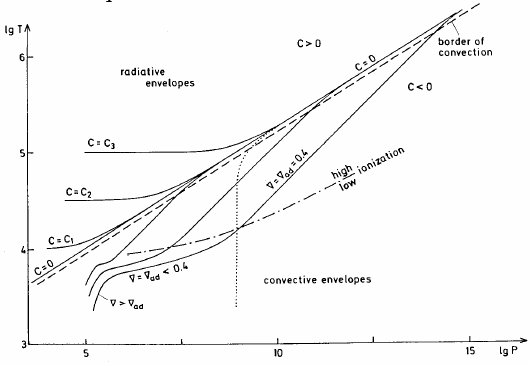
\includegraphics[trim={0cm 0cm 0cm 0cm},clip, keepaspectratio,width=0.99\textwidth]{envelopelnTlnP}\label{fig:envelopelnTlnP}
\end{figure}
\end{column}
\end{columns}
\end{frame}

\begin{frame}{Simplified atmosferic model: grey atmosphere}
Atmosphere model: usually PP geometry and solve HE equation using non grey radiative transport and EOS and convection if needed
\begin{align*}
&\TDy{\tau}{P}=\frac{g}{\kappa}\tag*{HE using $\tau$ as indip var}\\
&T^4=\frac{3}{4}T_e^4(\tau+\frac{2}{3})\tag*{or solar $T(\tau)$ empirical relation}
\end{align*}
integration from $\tau\approx0$ where $T\approx0$, $P\approx0$ down to $\tau=\frac{2}{3}$ where $T=T_e$ - using shooting method.
\end{frame}

\begin{frame}{Chemical mixing: diffusion and convection}

\end{frame}


\subsection{Metodo di Henyey: modelli evolutivi}\linkdest{henyey}

\begin{frame}{Metodo di Henyey $[96]$}
N mass-shell with boundaries at $m_j$ $m_1=0,m_2=m',\ldots,m_N=M$
\begin{columns}[T]
\begin{column}{0.5\textwidth}
\begin{align*}
&\frac{r_{j+1}-r_j}{m_{j+1}-m_j}=\frac{1}{4\pi r_{j+1/2}^2\rho_{j+1/2}}\\
&\frac{P_{j+1}-P_j}{m_{j+1}-m_j}=-\frac{Gm_{j+1/2}}{4\pi r_{j+1/2}}\\
&\frac{L_{j+1}-L_j}{m_{j+1}-m_j}=\epsilon_n(T_{j+1/2},\rho_{j+1/2},X_{s,j+1/2})+!!!\\
&\frac{T_{j+1}-T_j}{m_{j+1}-m_j}=-\frac{T_{j+1/2}}{P_{j+1/2}}\nabla_{j+1/2}\frac{Gm_{j+1/2}}{4\pi r^4_{j+1/2}}
\end{align*}
\end{column}
\begin{column}{0.5\textwidth}
\begin{align*}
&(Y^1=r, y^2=P, y^3=T, y^4=L)\\
&E_j^{i=1,\ldots,4}=\frac{y_{j+1}^i-y^i_j}{m_{j+1}^i-m^i_j}\\
&-f_i(y_{j+1/2}^1,\ldots,y_{j+1/2}^4)=0
\end{align*}
$j=2,\ldots,N-2$: 4N-8 vincoli e le condizioni al bordo
\begin{align*}
&J=N: S_1=y_N^2-f_S(y_N^1,y_N^4)=0\\
&S_2:y^3_N-g_S(y_N^1,y_N^4)=0\\
&j=1: C_i(y^1_2,y_2^2,y_2^3,y_2^4,y_1^2,y_1^3)=0\\
&y_1^1=y_1^4=0
\end{align*}
\end{column}
\end{columns}
$4N-2$ equazioni in $4N-2$ incognite
\end{frame}

\begin{frame}{Metodo di Henyey: solve system of algebraic equations}
\'A la Newton-Rapshon - Trial solution (solution at step $t-\Delta t$): $(S_i)_1\neq0$, $(C_i)_1\neq0$, $(E_i^j)_1\neq0$ so we have to find correction to trial solution $(y_i^j)_2=(y_i^j)_1+\delta y_i^j$ - by Taylor expansion we can express $\delta S_i$, $\delta C_i$, $\delta E^i_j$ as function of the unknown small correction:
\begin{align*}
&(S_i)_1+\delta S_i=0, (C_i)_1+\delta C_i=0, (E_i^j)_1+\delta E_i^j=0\\
&\left\{\begin{array}{l}\TDy{y_N^1}{S_i}\delta y_N^1+\TDy{y_N^2}{S_i}\delta y_N^2+\TDy{y_N^3}{S_i}\delta y_N^3+\TDy{y_N^4}{S_i}\delta y_N^4=-(S_i)_1\\
\TDy{y_2^1}{C_i}\delta y_2^1+\ldots+\TDy{y_2^4}{C_i}\delta y_2^4+\TDy{y_1^2}{C_i}\delta y_1^2+\TDy{y_1^3}{C_i}\delta y_1^3=-(C_i)_1\\
\TDy{y_j^1}{E_j^i}\delta y_j^1+\ldots+\TDy{y_j^4}{E_j^i}\delta y_j^4+\TDy{y_{j+1}^1}{E_j^i}\delta y_{j+1}^1\ldots+\TDy{y_{j+1}^4}{E_j^i}\delta y_{j+1}^4=-(E_j^i)_1\\
\end{array}\right.
\end{align*}
con $i=1,\ldots,4$, $j=2,\ldots,N$: sistema algebrico di $4N-2$ equazioni in $4N-2$ $\delta y_j^i$ incognite ha matrice dei coefficienti (\keyword{Henyey matrix}) non-zero only near the diagonal e determinante non nullo - soluzione con metodi algebrici standard - fisso $\epsilon>0$ accuratezza con cui voglio risolvere le equazioni della struttura stellare e ripeto la procedura finch\'e $S_i<\epsilon$, $C_i<\epsilon$ - local errors doesn't propagate to other mesh
\end{frame}

\subsection{Metodo di shooting: soluzione primo modello stellare con condizioni al bordo}\linkdest{shooting}

\begin{frame}{Step temporale e problema modello iniziale}
Step temporale $\Delta t$: uso metodo di Henyey per determinare le nuove abbondanze with I equations as I elements accounted for.
\keyword{Problem of first model}: i) Turn on $\epsilon_g$ within few models ii) Initial model of evolutionary sequence is evaluated with \keyword{shooting method}
starting from outer mesh with 4 boundary conditions for $T_e$, $L_s$, $P_s$, $R$ and using first order approx. $y_j^i=y_{j\pm1}^i+\TDy{m}{y_{j\pm1}}\,dm$: we determine $(y_f^i)_{surf}$ until some mesh f midway between center and surface and then integrate from centerup to $j=f$ using central trial conditions - we have $(y_f^i)_{center}\neq(y_f^i)_{surf}$ and have to correct trial central boundary conditions
\begin{columns}[T]
	\begin{column}{0.5\textwidth}
\begin{align*}
&\Delta(y_f^i)_{surf}=\TDy{y_N^1}{(y^i_f)_{surf}}\delta y_N^1+\TDy{y_N^4}{(y^i_f)_{surf}}\delta y_N^4\\
&\Delta(y_f^i)_{center}=\TDy{y_1^2}{(y^i_f)_{center}}\delta y_1^2+\TDy{y_1^3}{(y^i_f)_{center}}\delta y_1^3
\end{align*}
	\end{column}
	\begin{column}{0.45\textwidth}
correzione ai 4 valori al contorno $\delta y_N^1=\delta R$, $\delta y_N^4=\delta L_s$ e $\delta y_1^2=P_c$, $\delta y_1^3=T_c$ found solving \[-\Delta_f=\Delta(y_f^i)_{center}-\Delta(y_f^i)_{surf}\]
	\end{column}
\end{columns}
Fails in advanced stages when structure has strong gradient - In massive stars late phases we can't ignore acceleration term
\end{frame}
